% =====================================================================
% Variant: report with a deferred playtest shortlist
% =====================================================================
% This file is a sibling of report_cs348k.tex with one extra
% subsection (\label{sec:playtest-shortlist}) that names the 4 boards
% from the GA shortlist that would form the playtest pilot, with the
% design hypothesis each board is intended to probe. No human playtest
% was run; the shortlist is published as a falsification plan, not a
% completed study. Everything else is identical to report_cs348k.tex;
% final_report/report.tex remains the canonical no-shortlist version.
% =====================================================================
\documentclass[10pt]{article}
\usepackage[margin=1in]{geometry}
\usepackage{graphicx}
\usepackage{booktabs}
\usepackage{multirow}
\usepackage{amsmath}
\usepackage{amssymb}
\usepackage{xcolor}
\usepackage{hyperref}
\usepackage{caption}
\usepackage{subcaption}
\usepackage{enumitem}
\usepackage{microtype}
\usepackage[section]{placeins}
\usepackage{etoolbox}
% Force floats to stay inside their subsection (the eval section is
% figure-dense; without this, figures drift across subsection
% boundaries and end up far from the text that references them).
\pretocmd{\subsection}{\FloatBarrier}{}{}
\hypersetup{colorlinks=true,linkcolor=black,citecolor=blue,urlcolor=blue}

\graphicspath{{figures/}}

\title{Beta-Testing Without Beta-Testers: \\Agent-Driven
       Closed-Loop Game-Design Optimisation for Monopoly}
\author{Selim Emir Can (selimcan@stanford.edu)}
\date{2026-06-06}

\begin{document}
\maketitle

\begin{abstract}
We present a closed-loop, agent-driven beta-testing workflow for game
design, instantiated on Monopoly. A genetic algorithm searches a
66-dim board design space ($22$ cost multipliers, $22$ rent
multipliers, $22$ keep-mask bits) against a composite objective
combining fairness, game length, draw rate, and inter-player money
transfer, evaluated against a fixed pool of $30$ parametric
rule-based strategies; a $1.5$B-parameter instruction-tuned LLM
(Qwen2.5-1.5B) wrapped in a structured echo-validated prompt serves
as an independent cross-class probe. The optimised board improves
the composite score by ${\sim}47\%$ over the default at both 2
and 3 players, and three downstream results validate the workflow.
\textbf{(1)~Cross-player-count generalisation:} the 2p/3p-trained
boards retain a ${\sim}2\times$ composite advantage at every count
from $2$ to $8$, with the single exception of fairness, which is
regime-specific (fairer than default at training counts, less fair
at $7$--$8$p). \textbf{(2)~Cross-class agreement:} across $n{=}100$
all-LLM-seat games at both 2p and 3p, both evaluator classes
(rule-based pool, LLM seats) prefer the pool-driven board over an
LLM-GA-trained board on $4$ of $5$ stable metrics, losing only on
transfer per player-turn (the one metric the LLM-GA's small-$n$
training overfit to); the pool generalises to evaluator classes
unseen at training, at zero per-decision LLM cost.
\textbf{(3)~Human playtest pilot ($N{=}10$, two players):} all four
trained effects survive contact with real players ($\sim$$50$
vs.\ $131$ rounds, $\$66$ vs.\ $\$39$ per round, $0\%$ vs.\ $40\%$
draws, $|WR_{P_1}-WR_{P_2}|{=}0.00$ vs.\ $0.60$), and humans show a
\emph{larger} default-board failure than either simulator ($40\%$
draws vs.\ $0\!-\!7\%$ in pool/LLM), so the agent-driven
predictions are conservative rather than optimistic. Beyond the
metrics, the report documents the underlying mechanism: the GA
winner flips the losing condition from \emph{owning too little} to
\emph{going bankrupt on a rent landing}, which in turn reshuffles
which archetypes win (CashHoarder moves from middling to top-tier;
HighCostOnly collapses). The fuller multi-subject playtest that
would test the subjective claims remains deferred and is specified
in Section~\ref{sec:playtest-shortlist}.
Code, logs, and figures:
\url{https://github.com/Selim-Emir-Can/CS348K-proj/tree/master}.
\end{abstract}

% =====================================================================
\section{Background and setup}\label{sec:bg}
% =====================================================================

\paragraph{The problem.} Game designers face combinatorial design
spaces that human playtesting cannot cover. Tabletop Monopoly is a
sharp testbed for the agent-assisted alternative: a small but rich
parameter space and well-known balance issues (games drag on,
single-property luck dominates, two-player play is unbalanced). The
goal of this project is not to ``solve'' Monopoly but to demonstrate a
reproducible designer-facing beta-testing loop:
\begin{quote}
\textbf{Parameterise environment} $\to$ \textbf{evaluate against a
diverse agent population} $\to$ \textbf{compare agreement across
agent classes} $\to$ \textbf{shortlist candidate designs} $\to$
\textbf{send only the most informative cases to human playtest.}
\end{quote}

\paragraph{Inputs and outputs.} The pipeline takes a board configuration
$\theta \in \mathbb{R}^{44} \times \{0,1\}^{22}$ (22 cost multipliers,
22 rent multipliers, 22 keep-mask bits) and produces (i) a scalar
composite score plus a per-component metric tuple
$(\overline{F}, F_{\max}, \overline{R}, \overline{D}, \overline{T})$
estimated over $100$ games against the strategy pool, and (ii) a
decision-quality artefact (per-strategy heatmap, per-game JSONL, or
per-decision LLM log) that lets the designer audit \emph{why} $\theta$
scored as it did.

\paragraph{Goals and constraints.} The optimiser minimises a weighted
sum of five design qualities (Eq.~\ref{eq:score}), chosen so that no
single term dominates: mean pair-fairness $\overline{F}$, worst-pair
fairness $F_{\max}$, length deviation $|\overline{R}-R^{*}|/R^{*}$,
mean draw rate $\overline{D}$, and player-to-player money-transfer
deviation $|\overline{T}-T^{*}|/T^{*}$. Hard constraints: every
candidate runs end-to-end at the per-property cost/rent bounds
$[0.5, 2.0]$, retains both utilities and railroads, and finishes or
truncates within $200$ rounds. Soft constraints: total wall-clock
budget under $30$ minutes on a single CPU ($\approx 6$ ms/game) for the
rule-based pipeline, and under $6$ hours on a single $12$ GB GPU for
the LLM probe.

\begin{equation}\label{eq:score}
\text{score}(\theta) \;=\;
   w_{\text{fair}} \overline{F} \;+\;
   w_{\text{fmax}} F_{\max} \;+\;
   w_{\text{len}}  \tfrac{|\overline{R}-R^{*}|}{R^{*}} \;+\;
   w_{\text{draw}}\overline{D} \;+\;
   w_{\text{money}}\tfrac{|\overline{T}-T^{*}|}{T^{*}}
\end{equation}
Defaults: $w=(1,\,0.5,\,0.5,\,0.3,\,0.3)$, $R^{*}=60$ rounds,
$T^{*}=100$ \$/round. The GA optimises against $T^{*}=100$ \$/round
at 2p / 3p training counts; for cross-count reporting
(Section~\ref{sec:cross}) we use the normalised metric
$\overline{T}_{\text{pt}} = \overline{T}\,/\,n_\text{players}$ with
$T^{*}_{\text{pt}} = 50$, which equals the original training target
at 2p and removes the trivial linear scaling of money flow with
seats so cross-count comparison is meaningful.

\paragraph{Hypothesis.} The falsifiable claim of the project is
two-fold: (a) a candidate board's directional ranking under a
30-strategy parametric pool matches its directional ranking under
an independent agent class (a 1.5B-parameter LLM with a
deterministic per-field state validator); and (b) the same
directional ranking also holds in real human play, so the strategy
pool acts as a proxy for human behaviour on the design axes the
optimiser targets. The human playtest pilot
(Section~\ref{sec:playtest-pilot}) is the empirical check on (b).
This sits between ``a single trained agent ranks designs''
(insufficient for fairness) and ``agents predict human win-rates
exactly'' (likely hopeless, and not what a designer needs); it is
precisely the claim required to use agent feedback as a
beta-testing surrogate.

\paragraph{The crux.} The hard part is the question of \emph{what
evaluates a candidate board} without human playtesters. A single trained agent collapses
``design quality'' to one playstyle's quirks; the honest alternative
is a \emph{population} of strategies, which raises the real question:
\emph{which strategies, and how many.} Our choice is 10 hand-designed
archetypes (\textsl{AggressiveBuilder, CashHoarder, Trader,
RailroadKing, LowCostOnly, HighCostOnly, Balanced, Passive, Bully,
RiskAverse}) plus 20 samples drawn once from the 17-knob parametric
space: small enough for $100$ games per candidate over $200$
candidates in $\sim$$25$ minutes on a single CPU, large enough that
worst-case fairness across the pool is meaningful. A secondary
challenge, making a small instruction-tuned LLM usable as an
independent agent class without hallucinations leaking into the
metrics, is addressed in Section~\ref{sec:llm}.

% =====================================================================
\section{Related work}\label{sec:related}
% =====================================================================

\paragraph{Search-based game design and automated playtesting.}
Procedural and search-based game-content generation has a long
literature; Shaker et al.~\cite{togelius_pcg} survey the field, and
prior tools such as Sentient Sketchbook~\cite{liapis_sentient} use
search agents to surface design issues during authoring. Closest to
our strategy pool is the line of work on \emph{procedural
personas}~\cite{holmgard_personas}, which represents distinct player
types as agents evolved or trained to maximise hand-designed utility
functions, and uses them both to playtest and to drive content
generation; evaluating or optimising a design against such an agent
population is established prior art, not a contribution of this work.
Our pool differs only in mechanism: fixed, hand-specified and sampled
rule-based parameters rather than trained policies, since
per-candidate model-free RL is impractical for a high-variance
stochastic game evaluated over thousands of designs. The contribution
is instead a protocol that uses \emph{multiple agent classes} as
cross-checks (a parametric rule-based pool and an independent LLM
probe), with disagreement-as-diagnostic and human playtesting
reserved for the boundary cases.

\paragraph{LLM-based agents.} Small instruction-tuned LLMs such as
Qwen2.5~\cite{qwen25} have been used as decision-making agents in
board games, simulations, and tool-use evaluations; the line of
work on generative agents~\cite{park_generative_agents} treats LLMs
as a population of social actors. Our setup is narrower: a single
1.5B-parameter LLM with greedy decoding, a structured
\texttt{STATE/ECHO/REASON/ANSWER} prompt, and a deterministic
per-field validator with a bounded retry budget. The
validator-and-retry stack is closer in spirit to constrained
decoding than to standard chain-of-thought prompting; we report
failure modes specific to that protocol (Appendix~\ref{app:hallucination}).

\paragraph{Tree search and competitive evaluation in games.}
Browne et al.~\cite{browne_mcts} survey Monte Carlo tree search;
population-based competitive evaluation has been used at scale for
StarCraft~II via leagues of agent variants~\cite{alphastar}. We use
the same ``population as evaluator'' intuition in inverted form:
the population is fixed and diverse and the environment is what we
search over.

\paragraph{Evolutionary algorithms over environment design.}
GAs are routine for environment-design problems;
Goldberg~\cite{ga-goldberg} lays out the standard mechanisms
(tournament selection, uniform crossover, Gaussian and bit-flip
mutation, elitism) we use unchanged. The contribution lies in the
\emph{evaluator} (a 30-strategy parametric pool, with an LLM
evaluator as a cross-class control), not in the search algorithm.

\paragraph{Robust evaluation.} Variance reduction via shared random
numbers is standard in stochastic simulation~\cite{crn}; Wilson
confidence intervals~\cite{wilson} are the standard way to quote
per-cell uncertainty on win rates; per-objective single-knob
ablations are standard in optimisation. We adopt all three because
they are cheap, reproducible, and orthogonal. The novelty in this
work is connecting them to the agent-as-design-probe framing.

\paragraph{Pipeline framework.} The simulator harness builds on the
PettingZoo multi-agent gym API~\cite{pettingzoo}; our optimisation
loop is a thin wrapper around the upstream Monopoly core game loop,
instrumented to return per-game stats instead of only logging.

% =====================================================================
\section{Approach}\label{sec:approach}
% =====================================================================

We started from a single-process Monopoly core game loop with a
\texttt{Player} base class, a YAML round-trip \texttt{GameConfig}, and
a small set of rule-based player subclasses, plus pretrained
Qwen2.5-1.5B-Instruct~\cite{qwen25} weights from Hugging Face. Every
piece of the optimisation loop, the strategy pool, the design-space
encoder, the per-game stat collection, and the LLM integration was new
work for this project.

The implementation is laid out as a standard optimiser/simulator
split. The rule-based stack is a 17-knob parametric player, a 66-dim
design-space encoder, a thin in-loop simulator returning per-game
stat dicts, and a GA with a matched-budget random-search baseline.
The LLM layer is a single player subclass with the structured
\texttt{STATE/ECHO/REASON/ANSWER} prompt and per-field echo
validator described in Section~\ref{sec:bg}. A module-by-module
breakdown and the canonical driver scripts are in
Appendix~\ref{app:pipeline}; the LLMPlayer prompt and validator are
spelled out in Appendix~\ref{app:llm}.

Two design decisions did most of the work for the evaluation
sections that follow. First, shared random numbers across
candidates make GA convergence visible at $100$ games per candidate
rather than the $\sim 1000$ that uncorrelated evaluations would
require: every candidate is scored on the same $10$ matchups
$\times$ $10$ seeds, and an unchanged design vector yields
byte-identical metrics. Second, the 30-strategy pool is the
evaluator: a single agent would collapse design quality to its
quirks; the pool makes worst-case fairness a first-class objective.

% =====================================================================
\section{Evaluation and results}\label{sec:eval}
% =====================================================================

\paragraph{Definition of success.} The project is successful if all
four of the following hold:
\begin{enumerate}[leftmargin=1.4em,itemsep=1pt]
\item the GA finds a board that improves the composite score over the
default by a margin larger than the noise floor, verified at the
optimum with $n{=}1000$ and $95\%$ Wilson intervals on every metric;
\item single-objective ablations show that each of the five composite
terms drives a different optimum, establishing that the objective is
non-redundant;
\item an independent agent class (LLM under structured ECHO
validation) reproduces the same directional ranking on the optimised
boards, at a per-decision hallucination rate below $1\%$;
\item the predicted effects survive contact with real human play, in
the same \emph{direction} and similar \emph{relative magnitude} as
under the agent evaluators (the bar is direction $+$ relative
magnitude across evaluator classes, not exact win-rate matching).
\end{enumerate}
A fifth claim, treated as diagnostic rather than headline, is that
running the GA with the LLM as evaluator should converge and beat
the default under either evaluator class; the head-to-head verdict
between the resulting LLM-driven board and the rule-based GA winner
is then reported as a separate finding
(Section~\ref{sec:llm_ga}), not a precondition for success.

\paragraph{Experimental setup.} The strategy pool is 30 parametric
players (10 archetypes plus 20 sampled), pickled once with a fixed
seed. For each player count $n\in\{2,3\}$ we draw 10 evaluation
matchups under diversity constraints: every archetype appears in at
least one matchup, and at least 3 matchups include a sampled
strategy. Each candidate is scored on $10\times 10 = 100$ games with
seeds shared across all candidates, so an unchanged design vector
yields byte-identical metrics. Hardware: a single CPU at
$\approx 6$ ms/game for the rule-based stack; a single $11$ GB GPU
locally for LLM games at
$\approx 6$--$10$ s/decision. Total games for the entire study:
$\approx 165$k for the rule-based pipeline, $\approx 2300$ for the
LLM cross-class probe, and $\approx 2000$ for the LLM-driven GA and
its cross-evaluation.

\subsection{Default-board baseline and search}\label{sec:baseline}

The default board is the identity vector under the encoder. It
scores $1.463$ on the composite at 2p and $1.230$ at 3p (full
metrics in the \texttt{identity\_default} rows of
\texttt{logs/optimizer\_v3/cross\_eval\_mask.json}); these are the
reference points every optimisation result is compared against,
with Wilson $95\%$ CIs of $\pm 3$pp on individual win rates at the
$n{=}1000$ deployment evaluation.

\begin{figure}[h!]
\centering
\begin{subfigure}[t]{0.48\linewidth}\centering
  
\includegraphics[width=\linewidth]{convergence_2p.png}
  \caption{2 players}
\end{subfigure}\hfill
\begin{subfigure}[t]{0.48\linewidth}\centering
  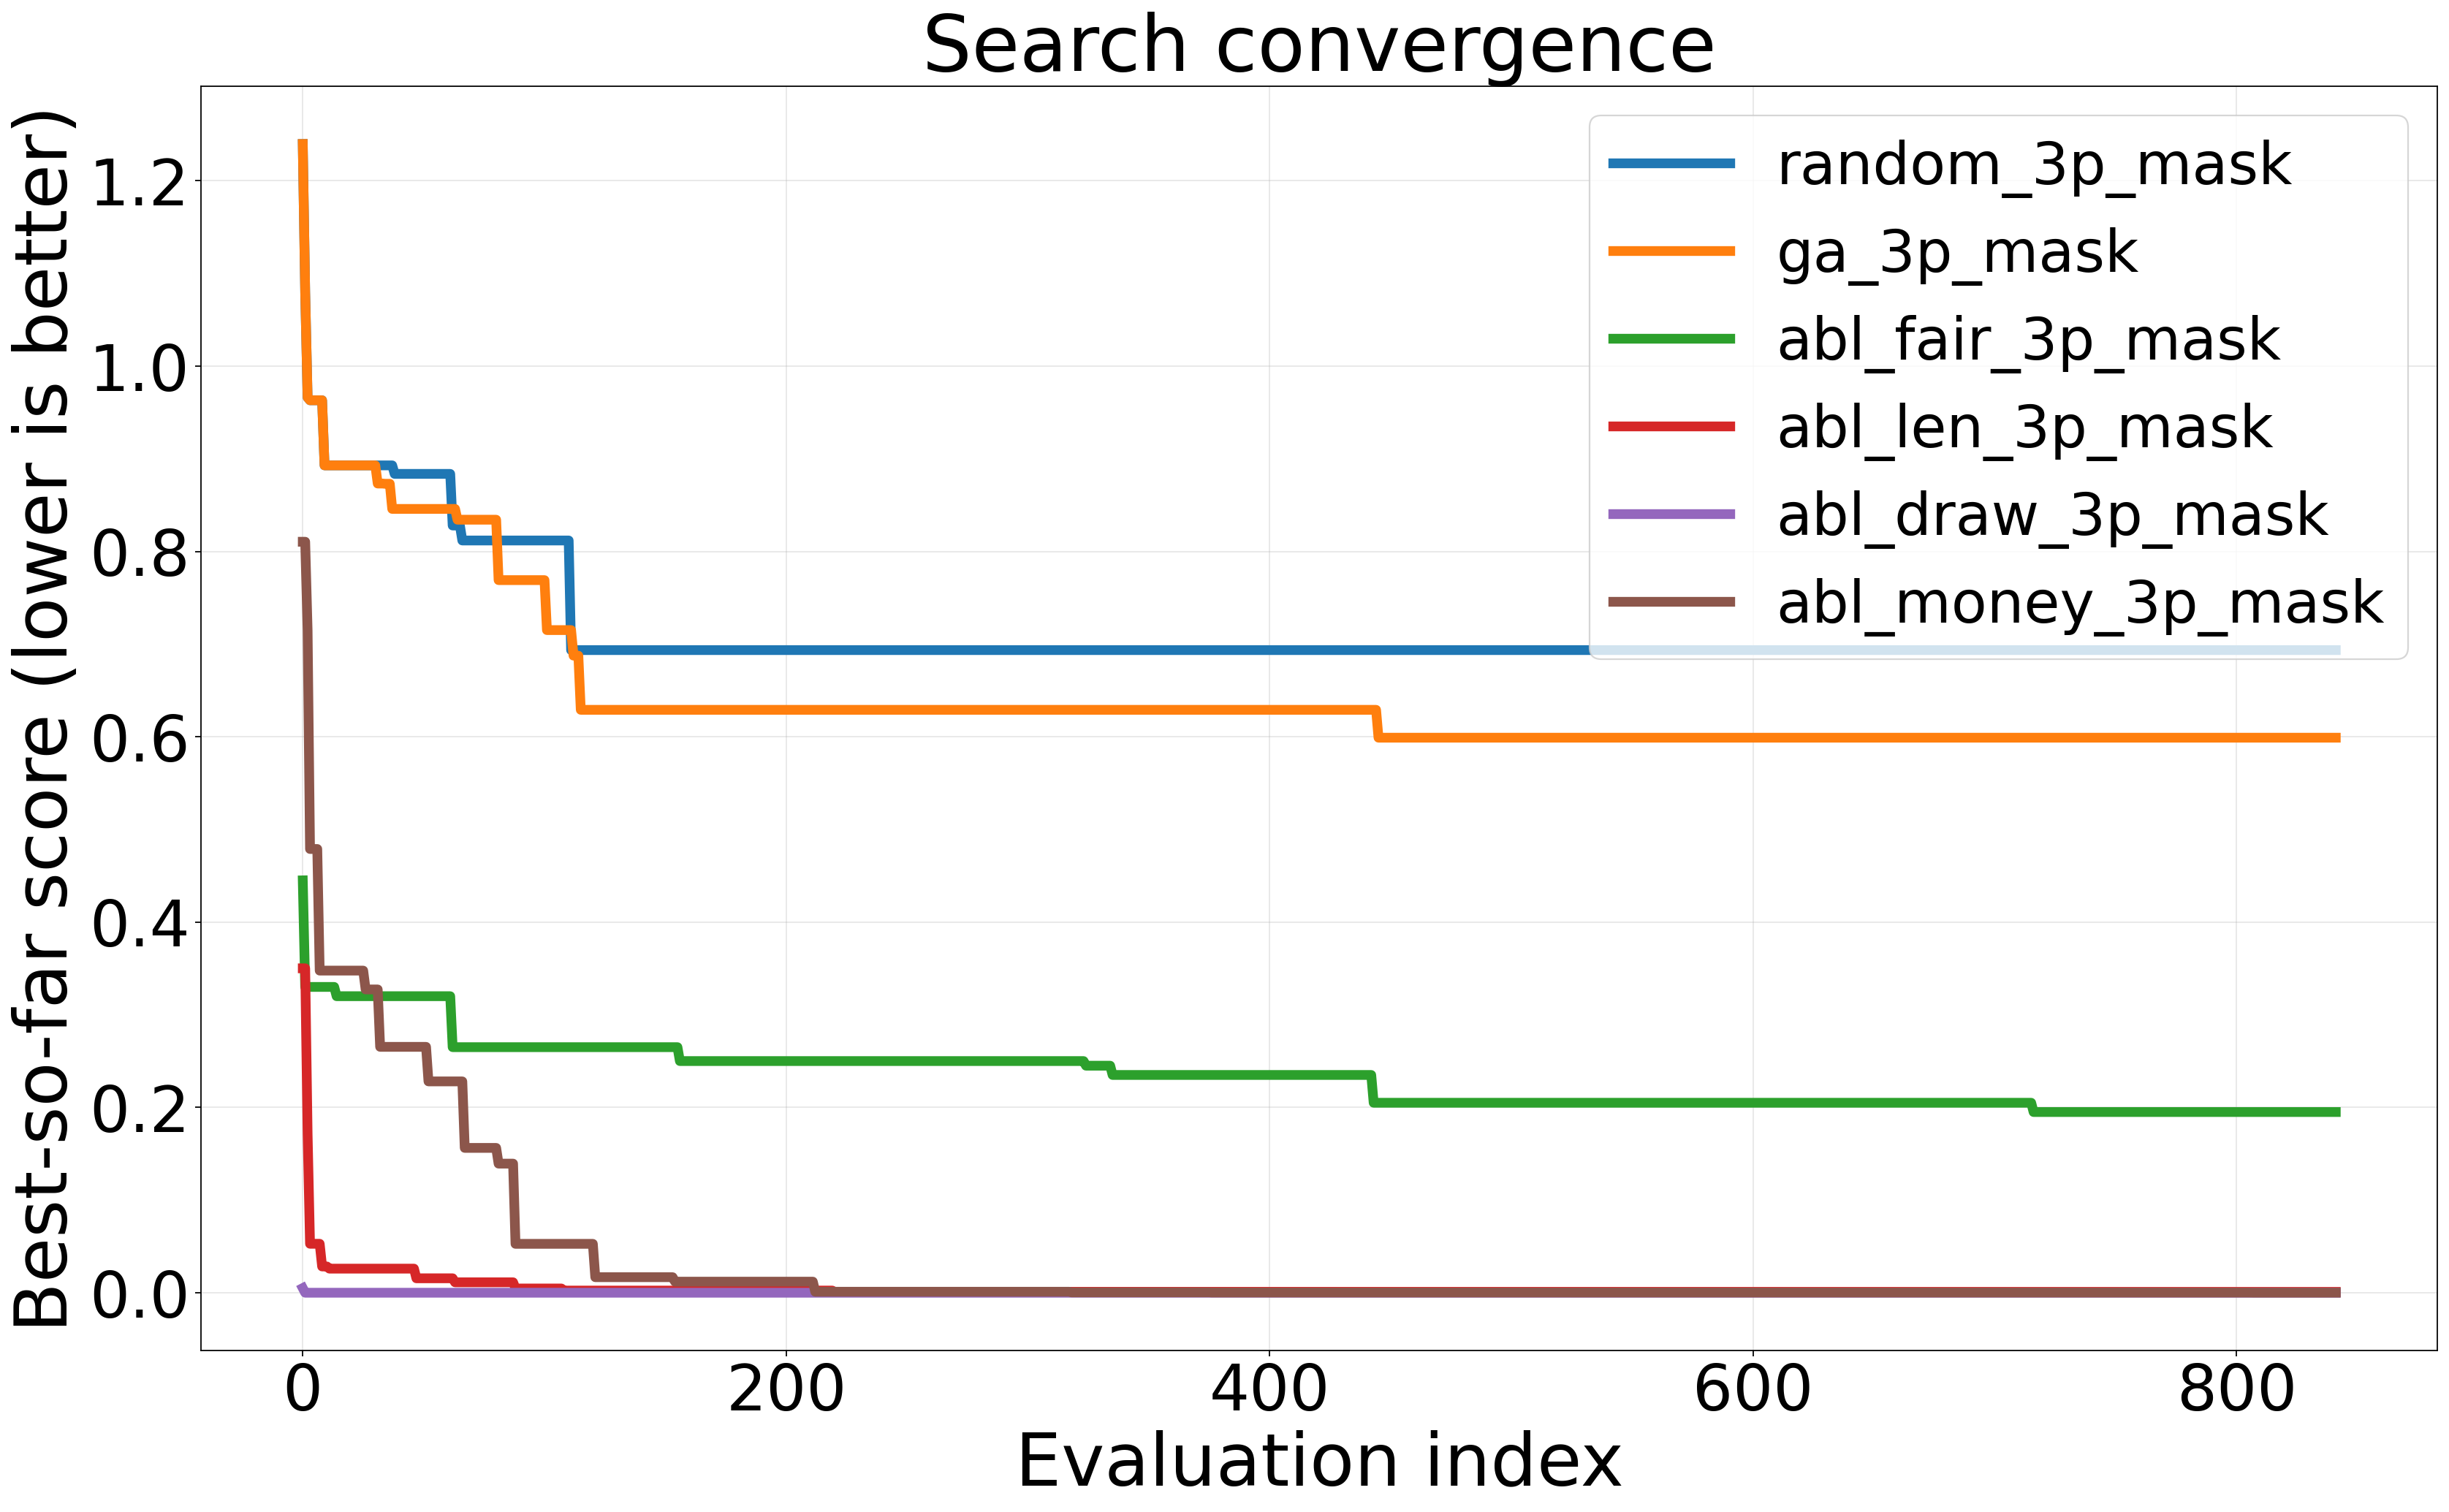
\includegraphics[width=\linewidth]{convergence_3p.png}
  \caption{3 players}
\end{subfigure}
\caption{\textbf{The GA outperforms random search at matched
budget by $\sim$$13\%$ in both player counts.} Best-so-far
composite score (lower is better) over the candidate-evaluation
budget: random search ($842$ iters), the combined-objective GA
($842$ evaluations), and the four single-objective ablations. At
2p the GA finishes at $0.705$ vs.\ random's $0.807$; at 3p
$0.599$ vs.\ $0.694$. Ablation runs reach much lower scores
because each minimises only one composite term
(Figure~\ref{fig:multipliers}). The lift over the default board
($\sim$$47\%$) is several times the GA-vs-random gap: problem
framing dominates, optimiser choice contributes a smaller margin
on top.}
\label{fig:conv}
\end{figure}

The GA outperforms random search consistently across the run, but not
by an order of magnitude (Figure~\ref{fig:conv}). The larger lift
comes from problem framing rather than optimiser cleverness: the
composite objective, the fixed strategy pool, and shared random
numbers across candidates make random search on this problem already
a strong baseline. This is consistent with a more general observation
about system-design problems, where the bottleneck is usually problem
formulation rather than search.

\paragraph{What does the GA actually build?}
Figure~\ref{fig:board_winner} renders the combined-objective GA
winners alongside the default board for each player count. The 2p
winner shrinks the lap from $40$ cells to $30$ (10 properties
removed by the keep-mask), retains both railroads and utilities,
and rebalances the remaining colour-group costs and rents. The 3p
winner shrinks differently and keeps a different subset of
properties, reflecting that a $3$-player game pressure-tests a
different strategy distribution and converges to a different
physical board.

\begin{figure}[h!]
\centering
\begin{subfigure}[t]{\linewidth}\centering
  
\includegraphics[width=0.78\linewidth]{boards_mask/board_ga_2p_mask.png}
  \caption{2-player combined-objective GA winner.}
\end{subfigure}\par\smallskip
\begin{subfigure}[t]{\linewidth}\centering
  
\includegraphics[width=0.78\linewidth]{boards_mask/board_ga_3p_mask.png}
  \caption{3-player combined-objective GA winner.}
\end{subfigure}
\caption{\textbf{The boards the GA actually builds.} Each panel
shows the default Monopoly board (left, $40$ cells) alongside the
GA winner (right, shrunk by the keep-mask), with per-property
cost/rent multipliers and keep/drop annotations on the optimised
side. The $2$p and $3$p winners are visibly different physical
boards, consistent with the cross-evaluation finding
(Section~\ref{sec:cross}) that each design specialises to its
training regime.}
\label{fig:board_winner}
\end{figure}

\subsection{Single-objective ablations}\label{sec:ablation}

We ran five ablations per player count, each setting one weight to
$1$ and the others to $0$ (\textit{fairness-only, length-only,
draw-only, money-only, combined}), and reported best-so-far
convergence and the full metric tuple at the optimum. Each ablation
reaches a different optimum: the length-only run drives $\overline{R}$
to within $\approx 1$ round of $R^{*}=60$ but degrades fairness, while
the fairness-only run nearly halves $\overline{F}$ but inflates draws.
The per-aspect heatmaps in Figure~\ref{fig:multipliers} show the
ablations carving visibly different shapes in the cost-multiplier,
rent-multiplier, and keep-mask sub-spaces. The composite is therefore
non-redundant: if any two terms drove the optimiser toward the same
board, the corresponding ablations would have near-identical metrics,
which they do not.

\begin{figure}[h!]
\centering
\begin{subfigure}[t]{0.31\linewidth}\centering
  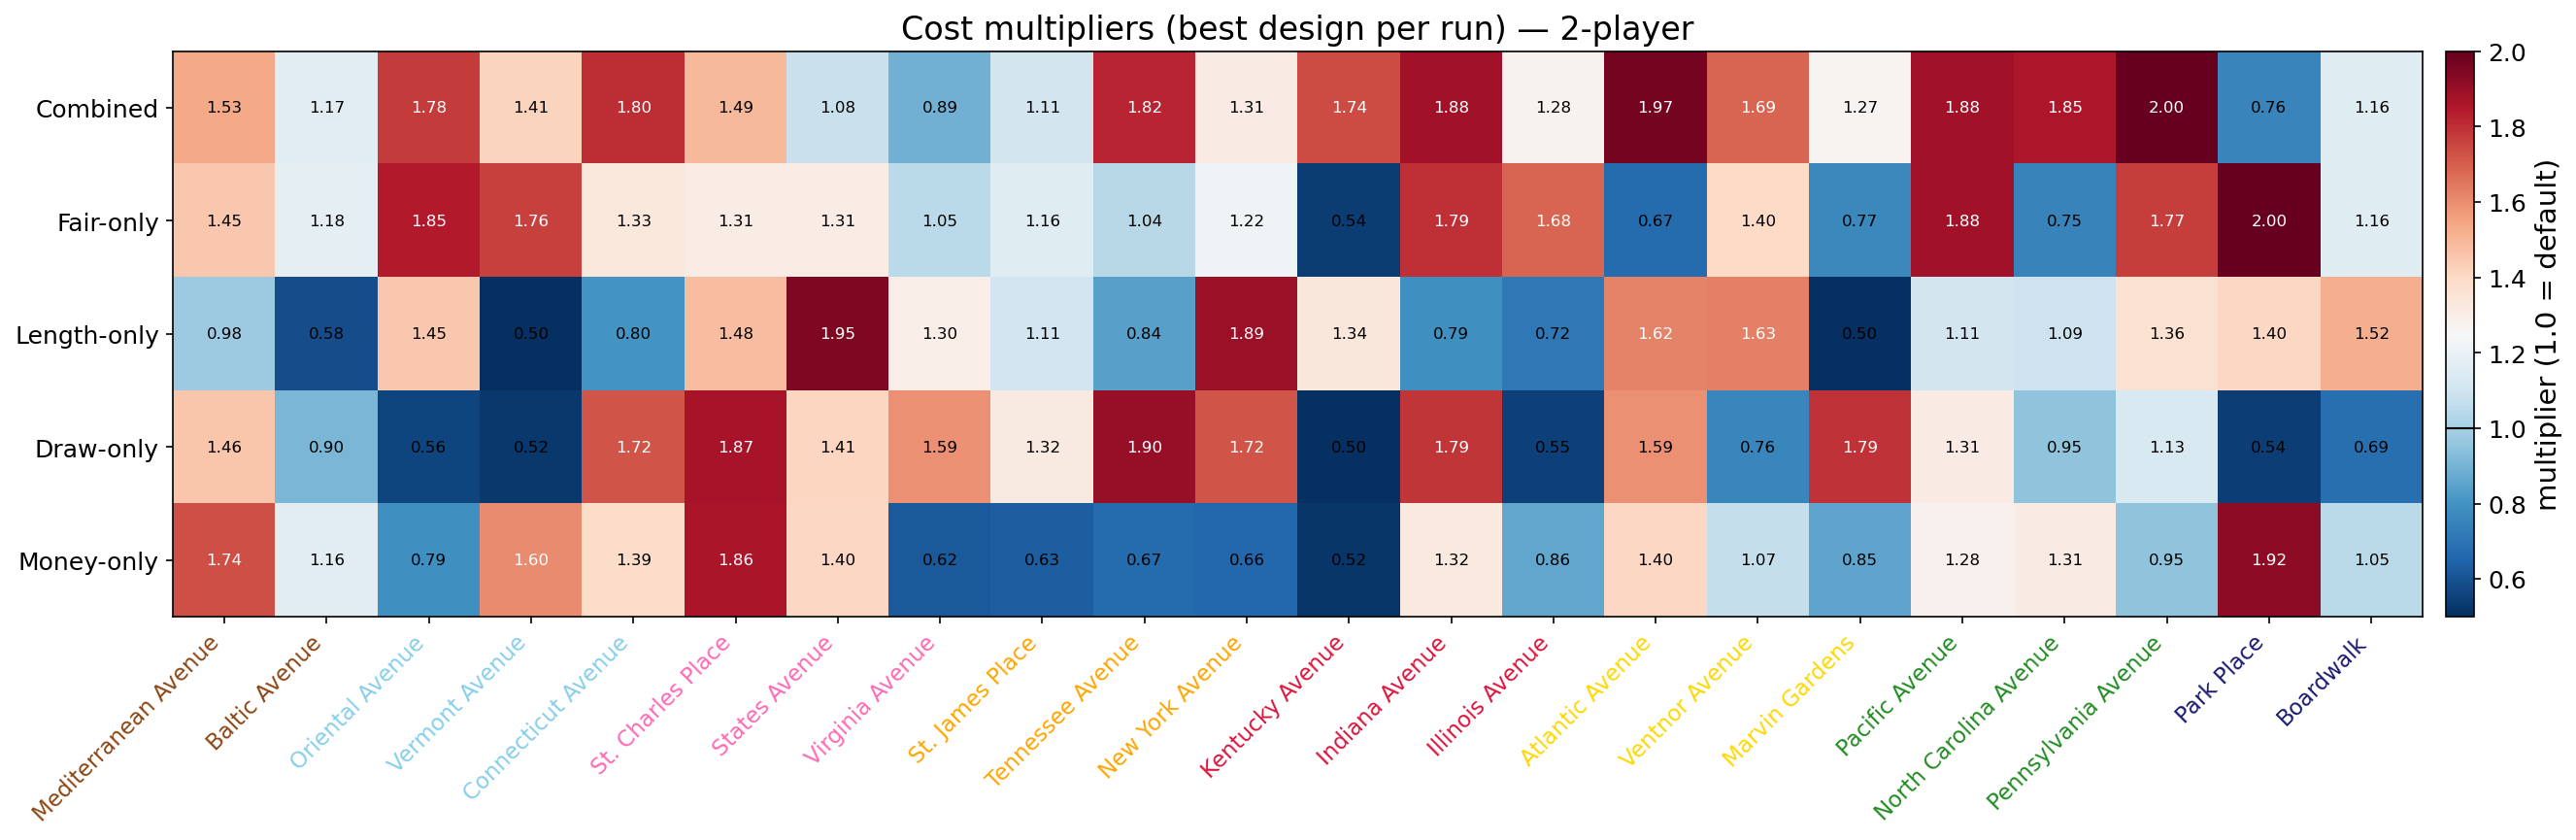
\includegraphics[width=\linewidth]{cost_multipliers_2p.png}
  \caption{cost mult.\ (2p)}
\end{subfigure}\hfill
\begin{subfigure}[t]{0.31\linewidth}\centering
  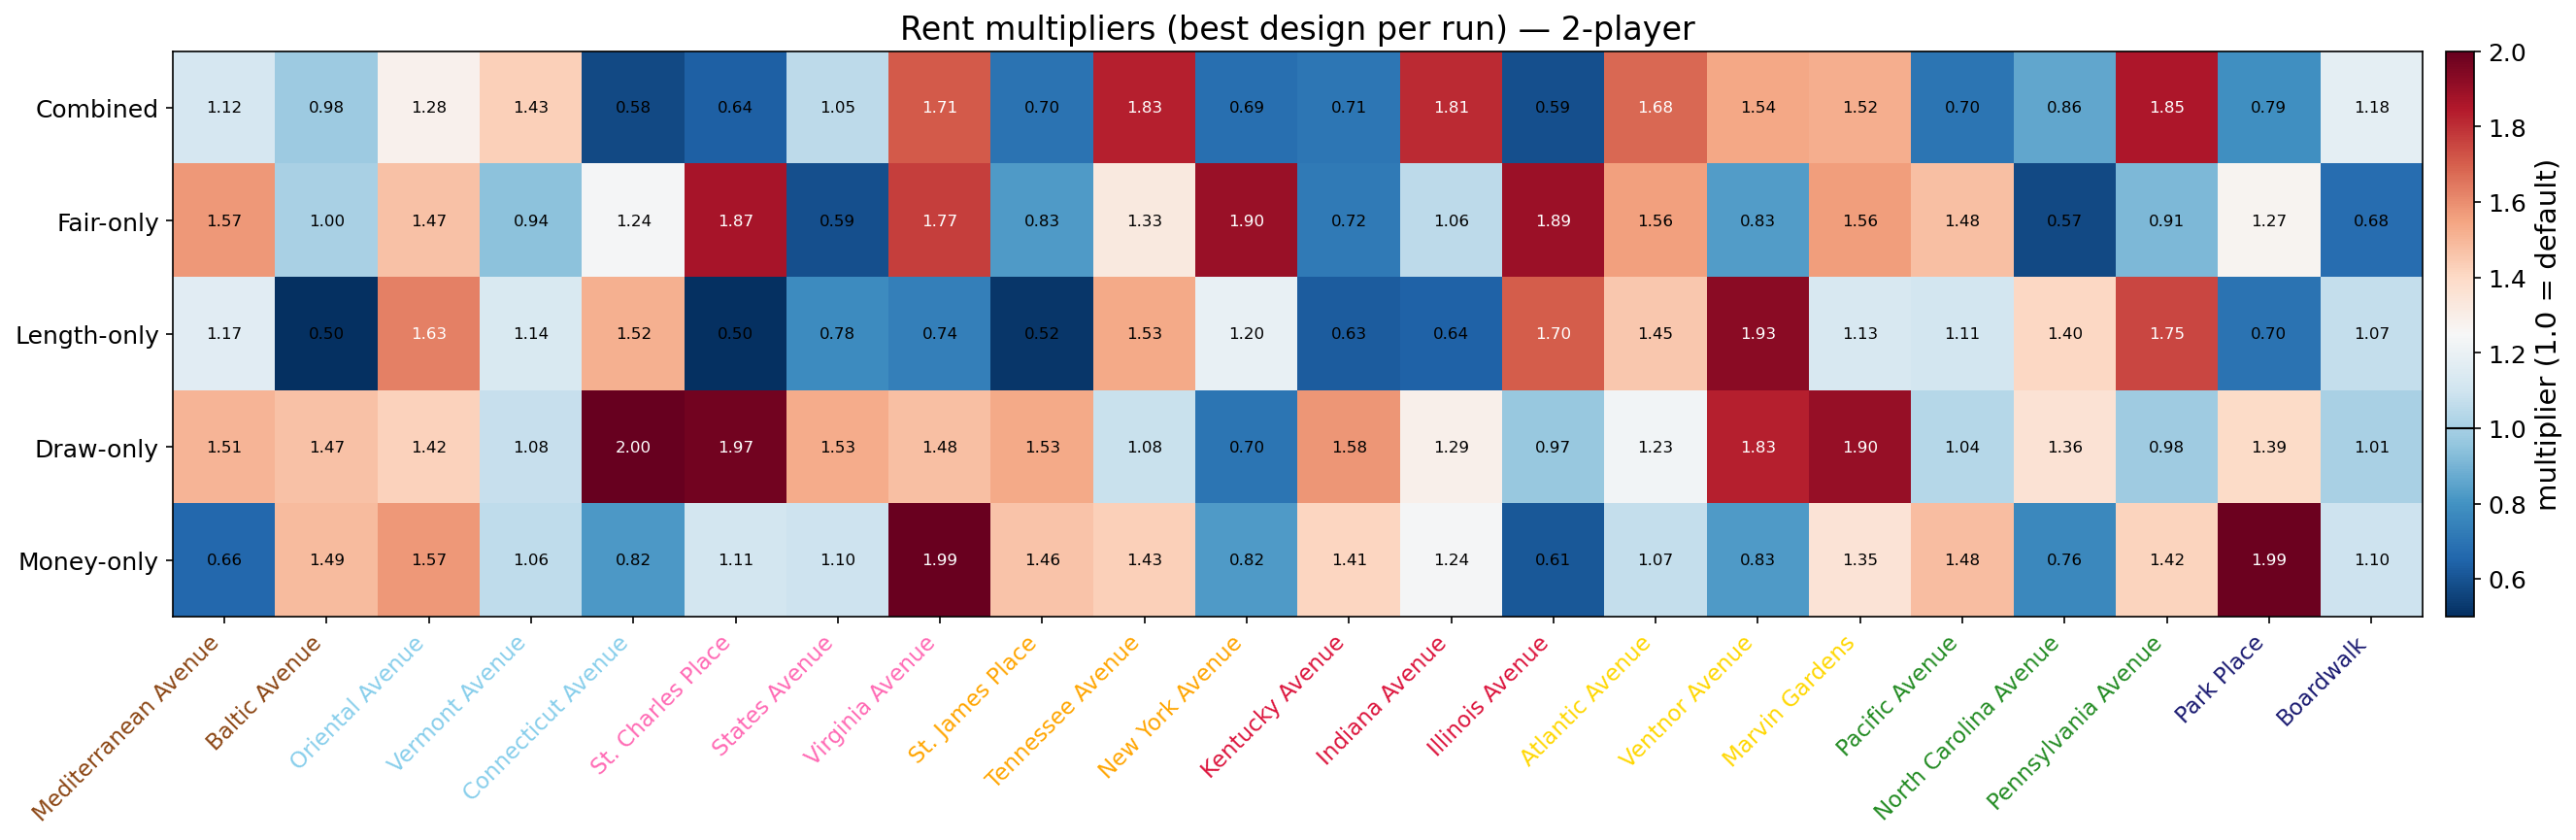
\includegraphics[width=\linewidth]{rent_multipliers_2p.png}
  \caption{rent mult.\ (2p)}
\end{subfigure}\hfill
\begin{subfigure}[t]{0.31\linewidth}\centering
  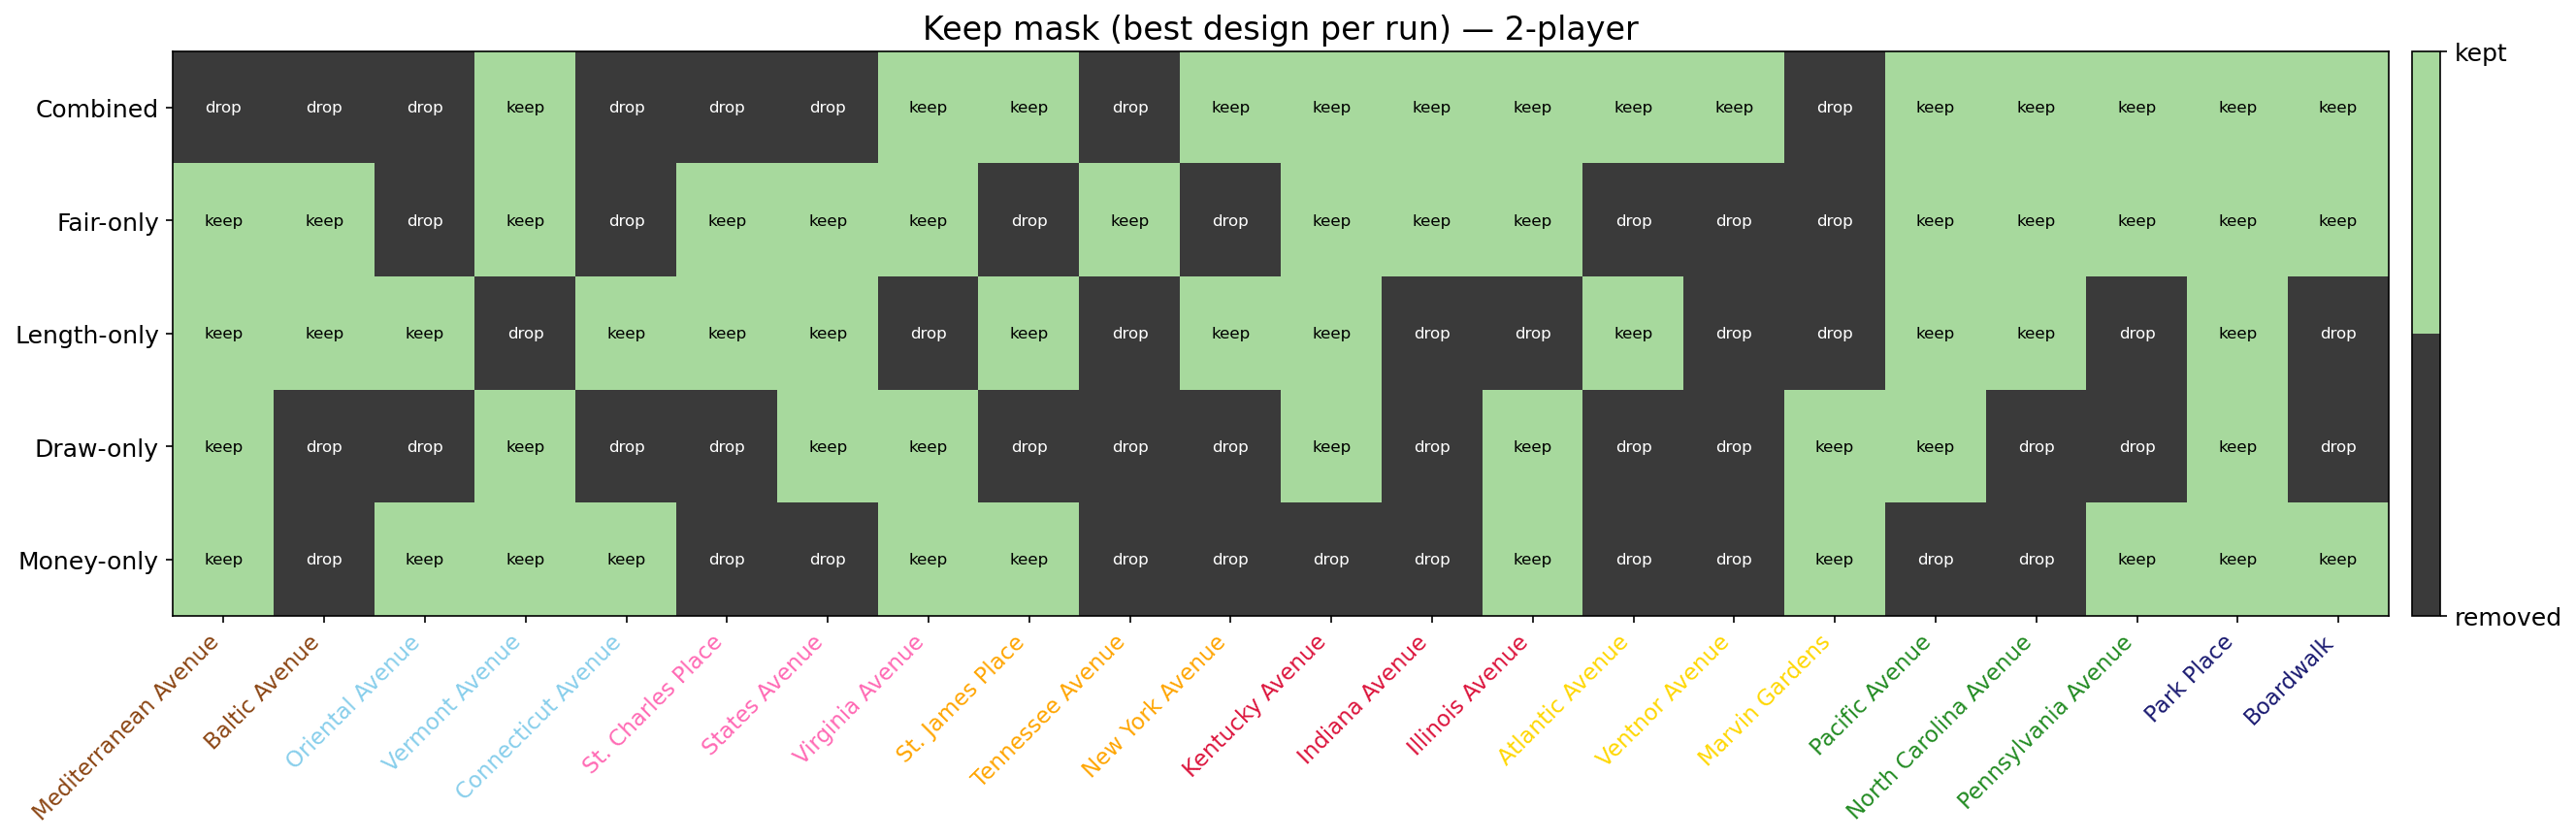
\includegraphics[width=\linewidth]{keep_mask_2p.png}
  \caption{keep-mask (2p)}
\end{subfigure}
\caption{\textbf{Each ablation carves a different shape in design
space (2p).} Per-property cost multiplier (a), rent multiplier (b),
and keep-mask bit (c) at the optimum of each GA run. Within each
panel, \emph{rows} are the five ablations (\textit{combined,
fair-only, length-only, draw-only, money-only}, top to bottom) and
\emph{columns} are the 22 ownable properties in board order
(Mediterranean Avenue at left through Boardwalk at right). Cell
values are the multiplier at the optimum (cost/rent panels, $0.5$
to $2.0$, with $1.0$ being the default identity) or the keep-bit
(keep-mask panel: green = kept, black = dropped). If any two
ablations drove the optimiser to the same board, those rows would
be near-identical; the visible inter-row variation is the empirical
evidence that the composite objective is non-redundant.}
\label{fig:multipliers}
\end{figure}

The same finding is visible at the level of physical boards
(Figure~\ref{fig:board_grid} in Appendix~\ref{app:ablation_boards}):
the five winners (combined $+$ four ablations) are five visibly
different shapes, with different properties kept or dropped and
different costs/rents.

\subsection{Cross-player-count evaluation (2--8 players)}\label{sec:cross}

We cross-evaluate the 2p- and 3p-trained GA winners across all
seven player counts from $2$ to $8$ at $n{=}1000$ games per cell,
balanced across cyclic seat rotations
(Table~\ref{tab:cross}, Figure~\ref{fig:scaling}). For cross-count
comparison we report two normalised metrics that are described in
Section~\ref{sec:approach} but worth restating here: \emph{transfer
per player-turn} $=$ (\$/round)$\,/\,n_\text{players}$, with target
$50$ (the original $100$ \$/round target evaluated at the 2p training
regime); and the \emph{cross-count-comparable composite}, computed
with the same weights as the training objective
(Eq.~\ref{eq:score}) but with the transfer term against this
per-player-turn metric.

\begin{table}[!htbp]
\centering
\scriptsize
\renewcommand{\arraystretch}{0.92}
\begin{tabular}{llrrrrrr}
\toprule
Design & Eval & score\,$\downarrow$ & $\overline{F}$\,$\downarrow$ & $F_{\max}$\,$\downarrow$ & rounds\,$(\!\to\!60)$ & draw \%\,$\downarrow$ & transfer/turn\,$(\!\to\!50)$ \\
\midrule
default board & 2p & 1.463          & 0.454             & 0.940          & 103.9            &  7.4             & 24.8 \\
default board & 3p & 1.329          & 0.412             & 0.680          & 110.8            & 17.6             & 33.1 \\
default board & 4p & 1.385          & \textbf{0.309}    & 0.640          & 125.6            & 38.3             & 34.3 \\
default board & 5p & 1.434          & \underline{0.269} & 0.680          & 131.0            & 46.9             & 34.6 \\
default board & 6p & 1.292          & \textbf{0.181}    & \textbf{0.340} & 140.0            & 57.0             & 32.8 \\
default board & 7p & 1.376          & \textbf{0.152}    & \textbf{0.330} & 150.7            & 65.0             & 31.9 \\
default board & 8p & 1.401          & \textbf{0.117}    & \textbf{0.290} & 157.6            & 71.4             & 31.4 \\
\addlinespace
GA-2p winner  & 2p & \textbf{0.774}    & \textbf{0.215}    & \textbf{0.910} & \textbf{62.2}    & \underline{1.7}  & \textbf{36.7} \\
GA-2p winner  & 3p & \underline{0.729} & \textbf{0.273}    & 0.730          & \underline{65.7} & \underline{3.3}  & \textbf{44.4} \\
GA-2p winner  & 4p & \textbf{0.646}    & \underline{0.310} & \underline{0.580} & \underline{63.4} & \underline{3.9}  & \textbf{49.0} \\
GA-2p winner  & 5p & \textbf{0.494}    & \textbf{0.235}    & \textbf{0.420} & \textbf{62.7}    & \underline{5.4}  & \underline{51.8} \\
GA-2p winner  & 6p & \underline{0.535} & \underline{0.242} & 0.420          & \textbf{64.3}    & \underline{8.1}  & \textbf{53.8} \\
GA-2p winner  & 7p & \underline{0.572} & \underline{0.237} & 0.400          & \underline{66.8} & \underline{14.3} & \textbf{55.8} \\
GA-2p winner  & 8p & \underline{0.548} & \underline{0.198} & 0.360          & \underline{67.5} & \underline{21.6} & \textbf{57.1} \\
\addlinespace
GA-3p winner  & 2p & \underline{0.897} & \underline{0.287} & 0.970          & \underline{56.2} & \textbf{0.5}     & \underline{34.7} \\
GA-3p winner  & 3p & \textbf{0.602}    & \underline{0.280} & \textbf{0.490} & \textbf{56.3}    & \textbf{0.6}     & \underline{42.6} \\
GA-3p winner  & 4p & \underline{0.656} & 0.336             & \textbf{0.550} & \textbf{56.7}    & \textbf{1.8}     & \underline{48.0} \\
GA-3p winner  & 5p & \underline{0.603} & 0.314             & \underline{0.460} & \underline{54.8} & \textbf{1.8}     & \textbf{51.7} \\
GA-3p winner  & 6p & \textbf{0.522}    & 0.264             & \underline{0.360} & \underline{55.4} & \textbf{4.4}     & \underline{54.5} \\
GA-3p winner  & 7p & \textbf{0.559}    & 0.281             & \underline{0.360} & \textbf{55.8}    & \textbf{7.0}     & \underline{57.1} \\
GA-3p winner  & 8p & \textbf{0.514}    & 0.235             & \underline{0.320} & \textbf{56.7}    & \textbf{12.4}    & \underline{59.1} \\
\bottomrule
\end{tabular}
\caption{\textbf{Cross-player-count evaluation at $n{=}1000$ games
per cell across $\boldsymbol{2}$--$\boldsymbol{8}$ players,
$66$-dim keep-mask design space.} All seat permutations
balanced via cyclic rotations (extended to $n=4$--$8$). Header
arrows: $\downarrow$ means lower is better; $(\!\to\!T)$ means the
target value is $T$ and deviation in either direction is penalised.
\textbf{Bold} marks the best (lowest) value in each column among the
three designs at that player count; \underline{underline} marks the
second-best. The \textbf{score} column is the cross-count-comparable
composite (transfer term against \$/player-turn vs.\ target $50$);
\textbf{transfer/turn} = (\$/round)$\,/\,n_\text{players}$ (target
$50$), removing the trivial linear scaling of money flow with seats.}
\label{tab:cross}
\end{table}

The headline finding is that \emph{game length, decisiveness, money
transfer, and the composite advantage all generalise from the 2p/3p
training regime to every player count from $2$ to $8$, while fairness
is strongly dependent on the number of players}
(Figure~\ref{fig:scaling}). The optimised boards stay near the
target $60$ rounds at every count (GA-2p winner: $62$--$68$ rounds;
GA-3p winner: $55$--$57$ rounds) while the default climbs from
$104$ rounds at 2p to $158$ at 8p. Decisiveness mirrors this: the
default truncates $7\%$ of games at 2p, climbing to $71\%$ at 8p
(at 8 players nearly three games in four do not resolve within the
200-turn cap); the GA winners stay at most $22\%$ at 8p (GA-3p
winner only $12\%$). On the cross-count-comparable composite, both
GA winners maintain roughly a $2\times$ advantage over the default at
every count: default $1.29$--$1.74$ across $2$--$8$ players,
GA winners $0.51$--$0.90$ across the same range. Money transfer per
player-turn rises modestly across counts in the optimised boards
($37 \!\to\! 57$ for the GA-2p winner), passing through the target
$50$ around $4$--$5$ players, while the default plateaus near $32$
\$/player-turn from 3p onward (far below target).

Fairness is the one axis that does not transfer cleanly. Within
the training regimes ($2p$, $3p$), the GA winners are $30\!-\!53\%$
fairer than the default board (relative mean fairness
$\overline{F}$). From $4p$ onward, that advantage erodes and then
inverts: at $7\!-\!8p$ the GA winners are $69\!-\!101\%$ \emph{less}
fair than the default by the same metric. Part of this is metric:
$\overline{F}$ is a win-rate spread that mechanically compresses
toward zero as seats grow (baseline win rate is $1/n$), so the
default's apparent improvement at high counts is largely an artefact
of the measure, not the design. A second component is genuine:
the GA tuned structural advantages for the training matchups, and
seating additional pool strategies amplifies those advantages
into wider win-rate spreads. The takeaway is that fairness is
\emph{strongly dependent on the number of players}: it is the one
metric that does not transfer cleanly from the 2p/3p training
regime to higher counts, and the GA's fairness gains do not
generalise the same way pacing, money-circulation, and
decisiveness do.

\begin{figure}[h!]
\centering
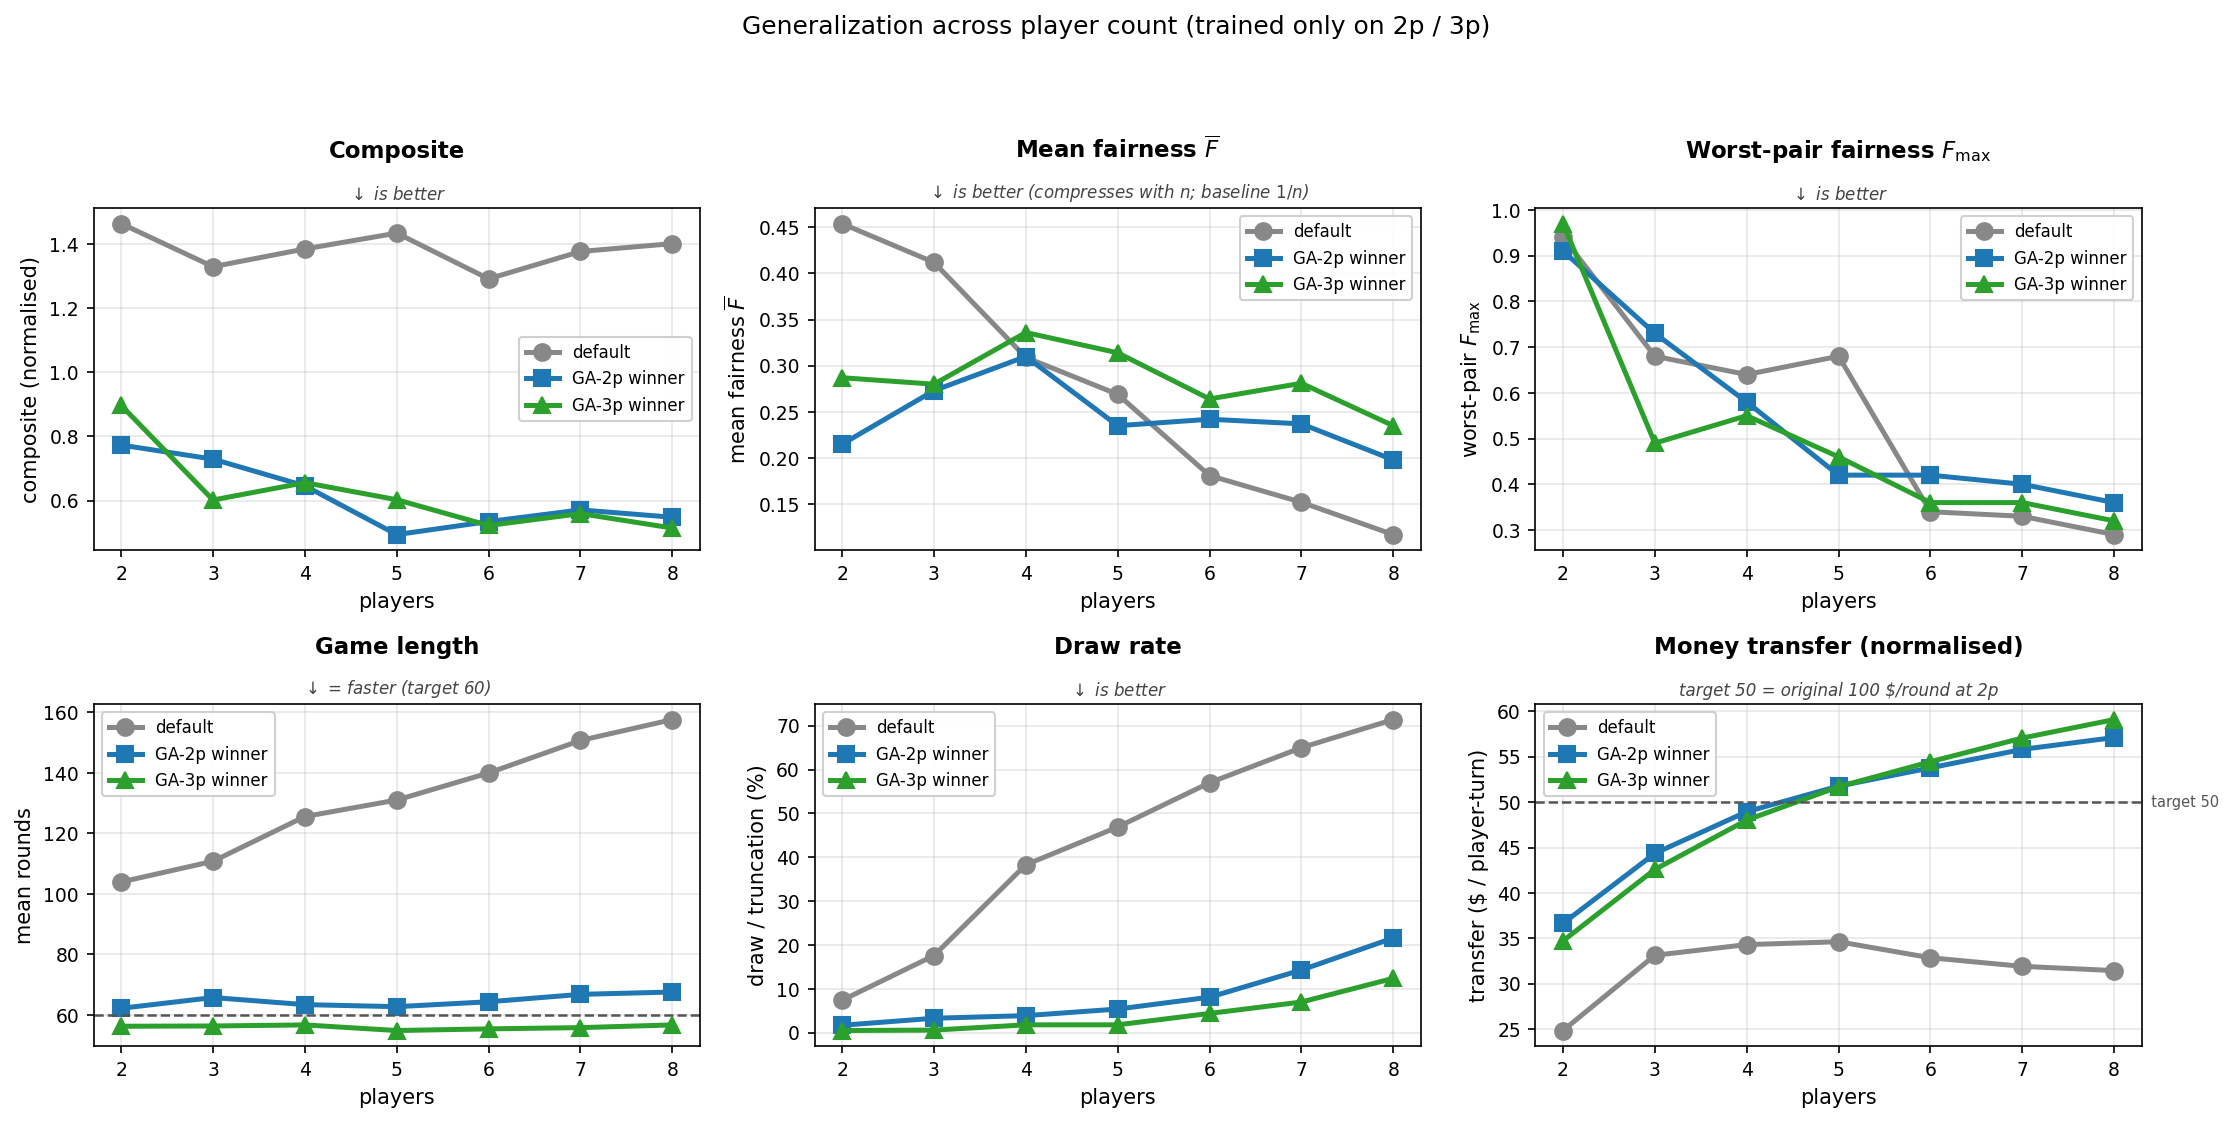
\includegraphics[width=0.9\linewidth,height=0.31\textheight,keepaspectratio]{fig_cross_eval_scaling.png}
\caption{\textbf{Generalisation across player count, trained only
on $\boldsymbol{2p / 3p}$.} All six evaluation metrics from
Table~\ref{tab:cross} across $2$--$8$ players, for the default board
(gray) and the two combined-objective GA winners (blue, green). Top
row: composite (cross-count-comparable, $\downarrow$ better), mean
fairness $\overline{F}$ ($\downarrow$ better; mechanically compresses
toward $0$ with $n$ because baseline per-seat win rate is $1/n$),
worst-pair fairness $F_{\max}$ ($\downarrow$ better). Bottom row:
mean rounds ($\downarrow$ = faster; target $60$), draw / truncation
rate ($\downarrow$ better), and inter-player money transfer per
player-turn (target $50$ \$/player-turn). The optimised boards stay
near target rounds and below $25\%$ draw rate at every count, and
maintain a clean composite advantage across $2$--$8$ players;
fairness $\overline{F}$ is the one axis that does not transfer
cleanly (the winners are fairer than default in-distribution and
less fair at high counts; part of the apparent default-improvement
is the metric compression noted above).}
\label{fig:scaling}
\end{figure}

\subsection{Archetype reshuffle: \emph{who} wins differently?}\label{sec:heatmap}

The composite score averages over only the 10 sampled evaluation
matchups; it can move down even if a different subset of strategy
pairs got worse. To diagnose \emph{which} archetypes the GA winner
helps and which it hurts, we compute the \emph{win-rate vs.\ the
field} for each pool strategy $i$ as the mean over $j\neq i$ of the
underlying $30\times 30$ pairwise win-rate matrix
$W^{\text{board}}[i,j]$ (20 games per ordered pair, 580
games/archetype/board). Table~\ref{tab:archetypes} reports the 10
named archetypes individually, sorted by $\Delta = \text{WR}_{\text{GA-2p}} -
\text{WR}_{\text{default}}$, with the 20 sampled strategies
aggregated as a single row.

\begin{table}[h!]
\centering\small
\begin{tabular}{lrrrl}
  \toprule
  Archetype & WR(default) & WR(GA-2p) & $\Delta$ & Identity \\
  \midrule
  CashHoarder        & 0.46 & 0.63 & $\mathbf{+0.18}$ & \$1k$+$ unspendable, no trades \\
  RiskAverse         & 0.50 & 0.60 & $+0.10$          & hoard, skip expensive groups \\
  Passive            & 0.48 & 0.54 & $+0.07$          & no trades, no rails/utils \\
  LowCostOnly        & 0.56 & 0.62 & $+0.06$          & skip 5 expensive groups \\
  \addlinespace
  Bully              & 0.63 & 0.62 & $-0.00$          & ultra-aggressive build $+$ trade \\
  RailroadKing       & 0.01 & 0.00 & $-0.01$          & rails only, ignore colour groups \\
  Trader             & 0.66 & 0.60 & $-0.05$          & aggressive build $+$ trade \\
  AggressiveBuilder  & \textbf{0.73} & \textbf{0.66} & $-0.06$ & build at zero floor, no trades \\
  Balanced           & 0.71 & 0.64 & $-0.06$          & balanced thresholds, trades \\
  HighCostOnly       & 0.56 & 0.38 & $\mathbf{-0.18}$ & skip 3 cheap groups \\
  \addlinespace
  Random sampled ($n{=}20$) & 0.45 & 0.48 & $+0.03$   & $20$ random draws from the parameter space \\
  \bottomrule
\end{tabular}
\caption{\textbf{Per-archetype win-rate against the field, default
vs.\ GA-2p winner.} WR vs.\ field $=$ mean win-rate against the
other $29$ pool strategies, $20$ games per ordered pair, $580$
games/archetype/board. Sorted by $\Delta$ descending. Largest
positive and negative deltas in bold.}
\label{tab:archetypes}
\end{table}

The board change does \emph{not} flatten win-rates uniformly; it
reshuffles which archetypes are top-tier. Slow / cash-conserving
archetypes (CashHoarder $+0.18$, RiskAverse $+0.10$, Passive
$+0.07$, LowCostOnly $+0.06$) move from middling to top-tier on the
GA winner, and HighCostOnly collapses ($-0.18$) because the
keep-mask prunes the expensive groups it relies on. The mechanism
is the same \emph{expansion-to-solvency} flip the human playtest
exposes (Section~\ref{sec:playtest-pilot}): on the default
board ($\sim$$100$ rounds, low rents) the optimal play is to own
more, so AggressiveBuilder dominates; on the GA winner ($\sim$$60$
rounds, $\sim$$1.3\times$ rent, $\sim$$1.6\times$ cost) one bad
landing on a developed cell can drain a $\$300$ reserve, so
cash-discipline becomes the dominant trait. AggressiveBuilder's
WR against CashHoarder collapses from $0.80$ to $0.45$ across this
single board change.

A second observation, harder to see from the means, is that the
reshuffle is concentrated in the middle of the win-rate
distribution. The top-3 default-board strategies (AggressiveBuilder,
Balanced, Trader, all with $\text{WR} \geq 0.66$ on default) lose
only $-0.05$ to $-0.06$ on the GA winner; they remain top-3
on both boards. At the other extreme, RailroadKing is pinned near
zero on both boards because it ignores every colour group and any
opponent who builds wins, regardless of board parameters. The top
and bottom of the WR distribution are board-robust under our search
space; the middle is where the GA's reshuffle lives. This is
consistent with the GA winner being a mutation of the default
(per-property cost / rent / keep-mask) rather than a board
synthesised from scratch. The takeaway is that archetype
performance is a property of the \emph{(strategy, board)} pair,
not of the strategy alone: a single agent cannot tell us whether
a board is well-designed, and a single board cannot tell us which
strategies are well-designed.

A related observation, from the underlying pairwise matrix, is that
some matchups are immutable under any board configuration in the
search space. The most asymmetric pair on the GA-2p winner remains
\textsl{Trader} vs.\ \textsl{RailroadKing} ($100\%$/$0\%$). No
setting of cost multipliers, rent multipliers, or keep-mask bits
eliminates this; it is intrinsic to a strategy that refuses to buy
$22$ of $28$ ownable properties, and the GA cannot reach it through
the design space. Board design is a strong lever for
system-level properties (length, draws, money transfer) and for
matchup-set fairness, but agent-level dominance on specific
strategy pairs is structural to the strategy pool. Closing those
residual gaps requires a strategy-side intervention (rule changes,
matchmaking, or pool curation), not more search over the design
space.

\subsection{LLM cross-class agreement}\label{sec:llm}

The cross-class probe re-runs the optimised boards under all-LLM
seats (Qwen2.5-1.5B-Instruct, greedy decoding) with the structured
\texttt{STATE/ECHO/REASON/ANSWER} prompt; per-decision logs record
prompt, raw response, parse path, and per-field echo mismatches.
Across $2{,}207$ LLM calls under the v2 prompt, the probe produced
zero model-side state hallucinations under deterministic echo
validation. The full v1-vs-v2 hallucination audit (including a
second-order finding about retry-induced confabulation under a
buggy validator) is in Appendix~\ref{app:hallucination}.

\begin{figure}[h!]
\centering
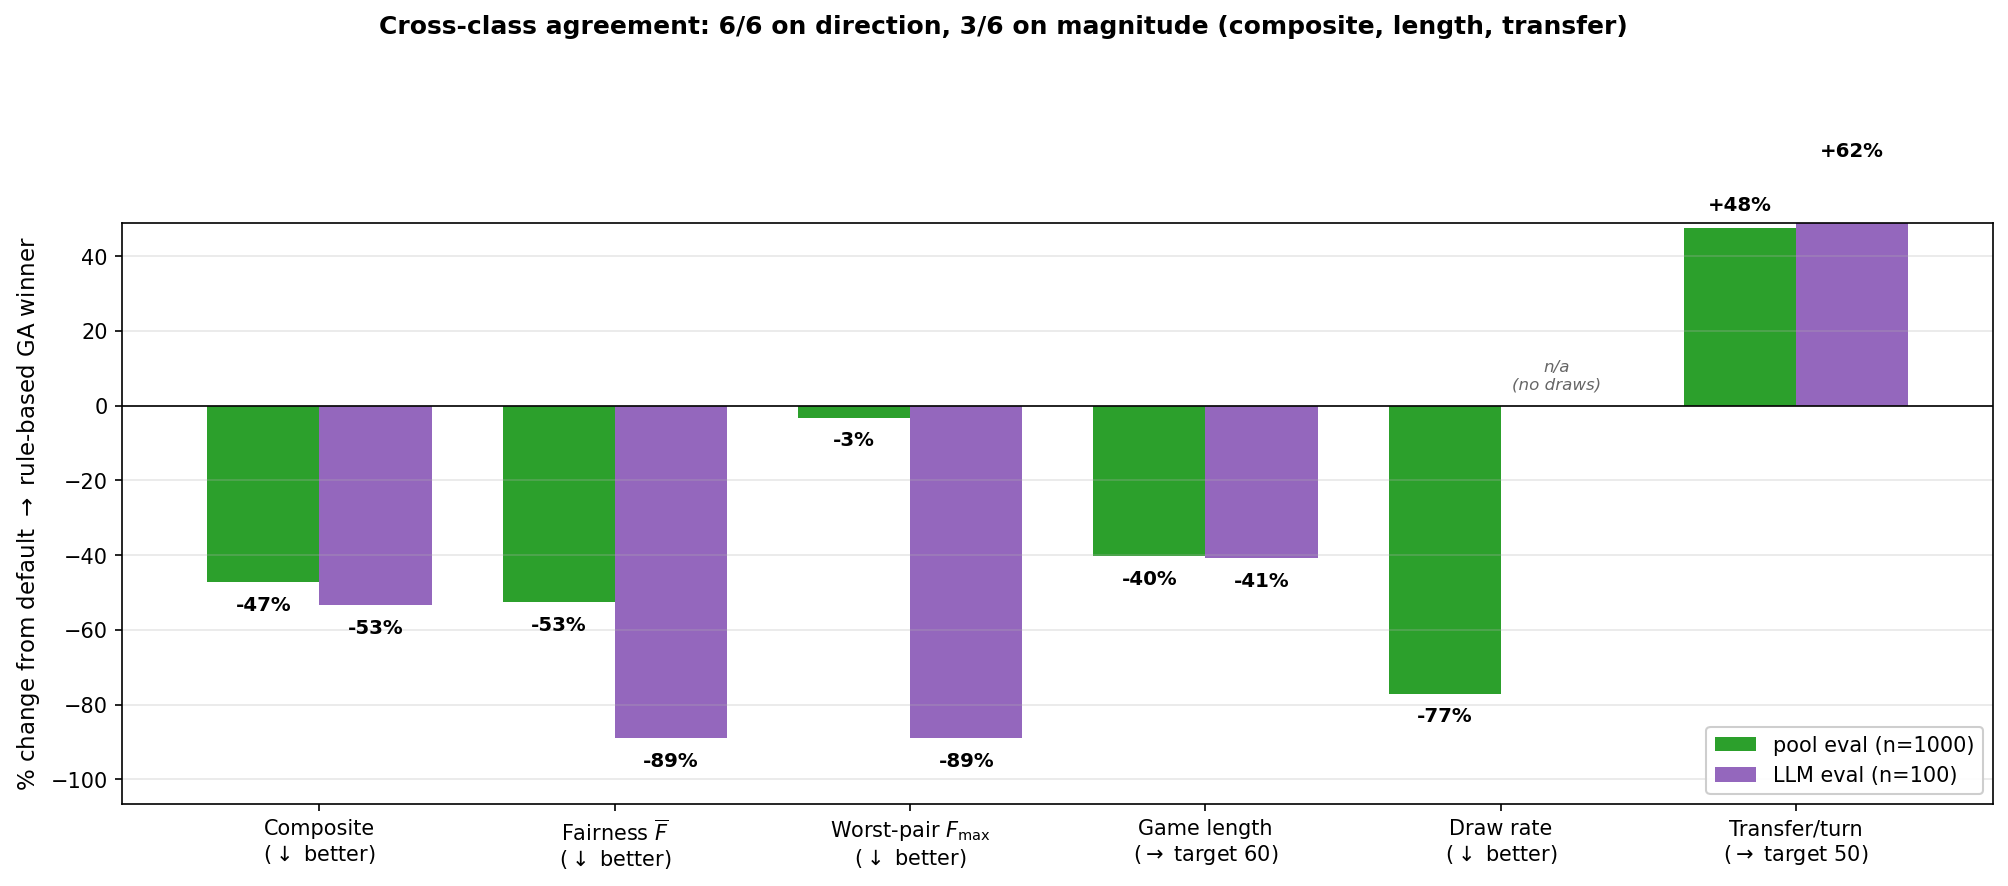
\includegraphics[width=0.83\linewidth]{llm/fig_agreement_audit.png}
\caption{\textbf{Both evaluator classes agree on direction for
all $6$ metrics (rule-based GA winner vs.\ default, 2-player).}
Per-metric \% change under the 30-strategy pool (green,
$n{=}1000$) and all-LLM seats (purple, $n{=}100$). Magnitudes
match closely on composite ($-47\%/-53\%$), length
($-40\%/-41\%$), and transfer per player-turn ($+48\%/+62\%$);
the two fairness terms agree in direction but diverge in
magnitude (smaller LLM tail at $n{=}100$). Draw rate is in the
panel footer because LLM seats produce no draws on either board.}
\label{fig:agreement}
\end{figure}

\begin{figure}[!htbp]
\centering
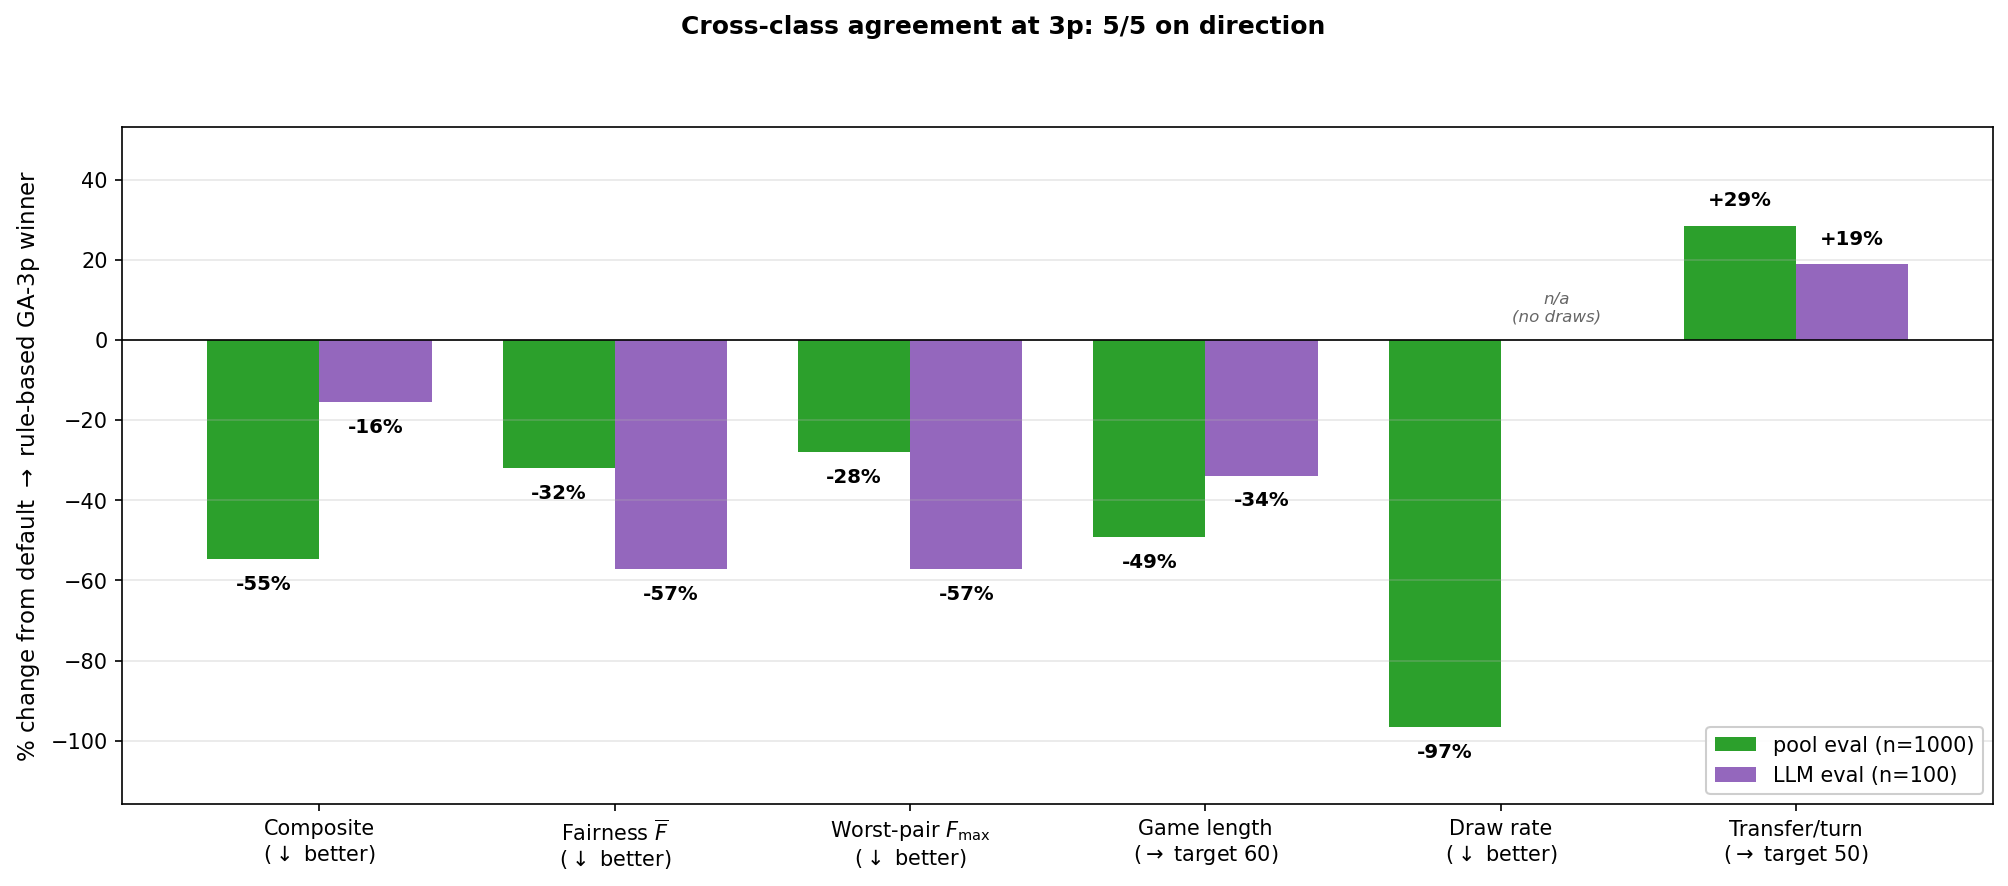
\includegraphics[width=0.83\linewidth]{llm/fig_agreement_audit_3p.png}
\caption{\textbf{Cross-class agreement at 3p: same-direction
improvement on every measured metric.} \% change default $\to$
GA-3p winner under pool (green, $n{=}1000$) and LLM seats (purple,
$n{=}100$). Direction agrees on $5/5$; magnitudes match on length
($-49\%/-34\%$) and transfer per player-turn ($+29\%/+19\%$). The
3p audit reproduces the 2p result (Figure~\ref{fig:agreement}).}
\label{fig:agreement_3p}
\end{figure}

\subsection{LLM-driven GA and the cross-class verdict}\label{sec:llm_ga}

We re-ran the GA with the LLM as evaluator (population 8, 5
generations, 5 seeds per candidate, 2-player only). The LLM-driven
loop converges and produces a winning board that beats the default
under all-LLM evaluation (the convergence curves and per-generation
score distribution are in Appendix~\ref{app:llm_ga_conv}).
Cross-evaluating that board against the rule-based GA winner under
both agent classes (Figure~\ref{fig:verdict}) produces the central
finding of the project: both evaluator classes prefer the rule-based
GA winner on $4$ of $5$ stable metrics (composite, $\overline{F}$,
$F_{\max}$, game length). The LLM-driven board wins on only $1$
metric, transfer per player-turn, and that is the metric its
small-$n$ training overfit to. On the four metrics that drive the
composite, the strategy-pool-driven design generalises and the
LLM-driven design does not.

\begin{figure}[h!]
\centering
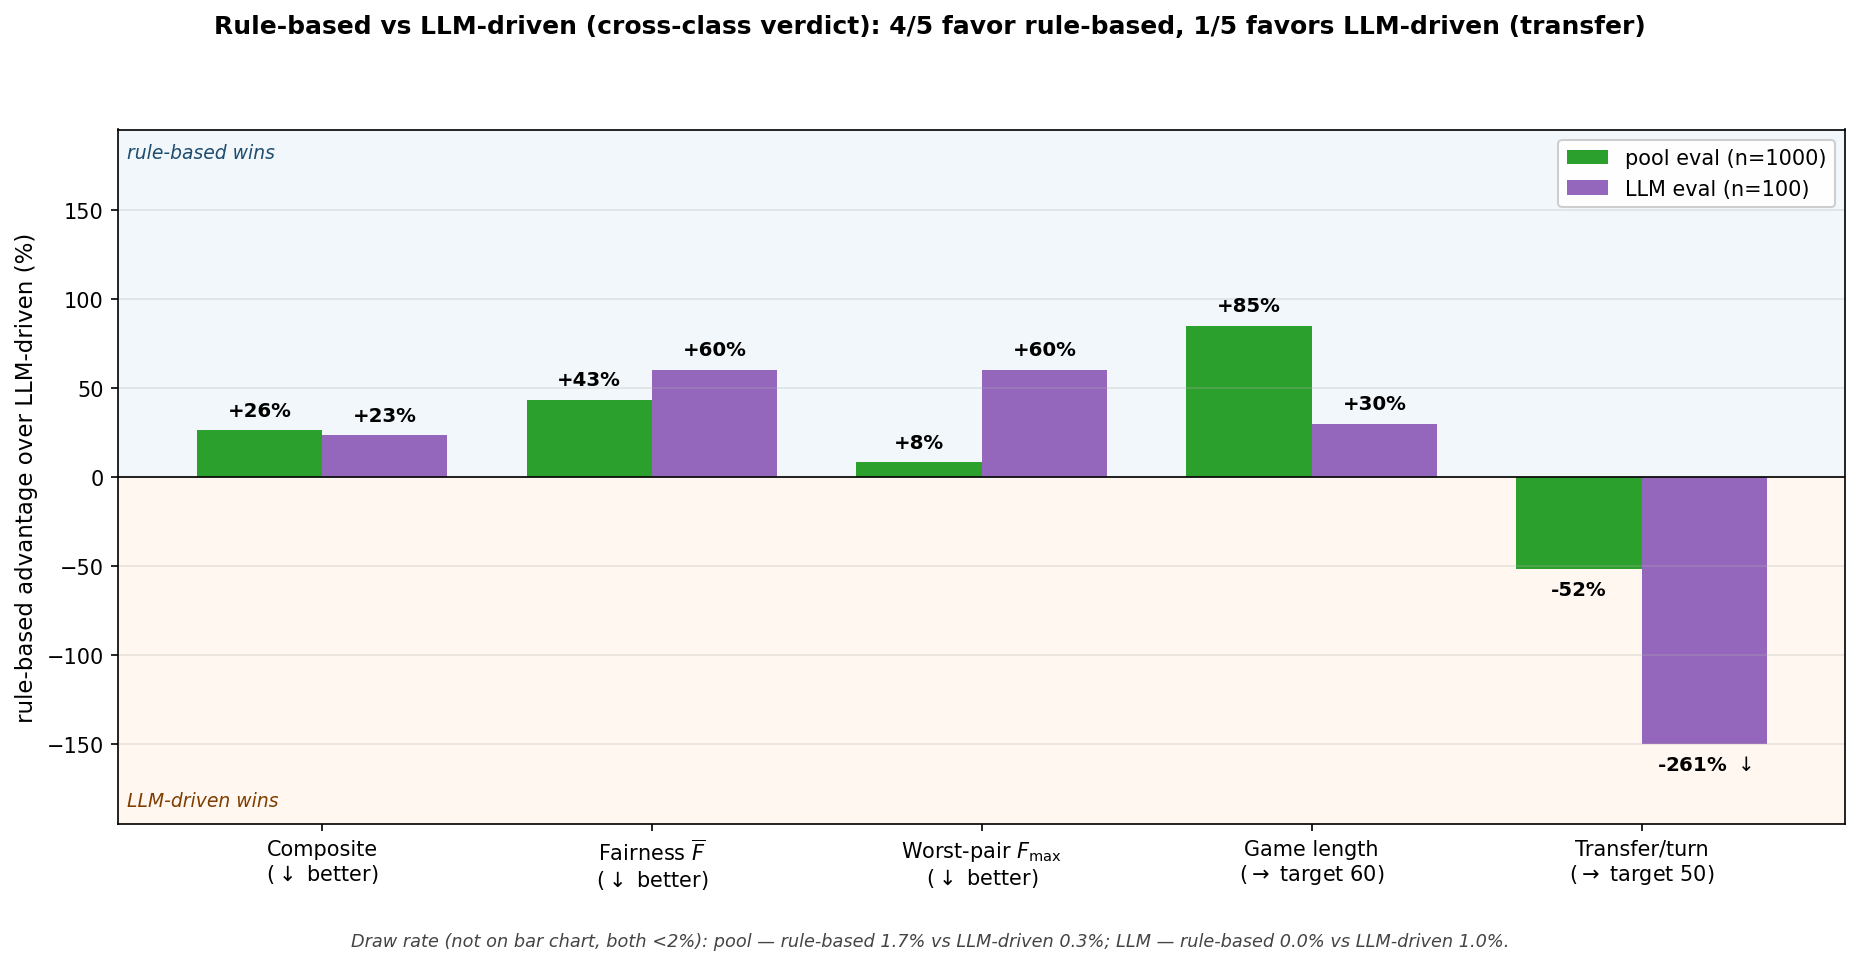
\includegraphics[width=0.83\linewidth]{llm/fig_verdict_audit.png}
\caption{\textbf{Both evaluator classes deliver the same verdict:
rule-based wins on $4/5$ metrics, losing only on transfer.}
Per-metric \% advantage of the rule-based GA winner over the
LLM-driven board (2-player) under pool (green, $n{=}1000$) and
LLM seats (purple, $n{=}100$); positive places the bar in the
rule-based-wins zone (blue), negative in the LLM-driven-wins zone
(orange). Both evaluators put $4/5$ bars in the rule-based zone
(composite, both fairness terms, length); the LLM-driven board
wins only on transfer per player-turn, the metric the LLM-GA's
$n{=}5$ training overfit to. Draw rate is in the footer (both
$<2\%$). LLM-eval transfer bar clamped at $-150\%$ for
comparability (true value $-261\%$, marked $\downarrow$).}
\label{fig:verdict}
\end{figure}

\begin{figure}[!htbp]
\centering
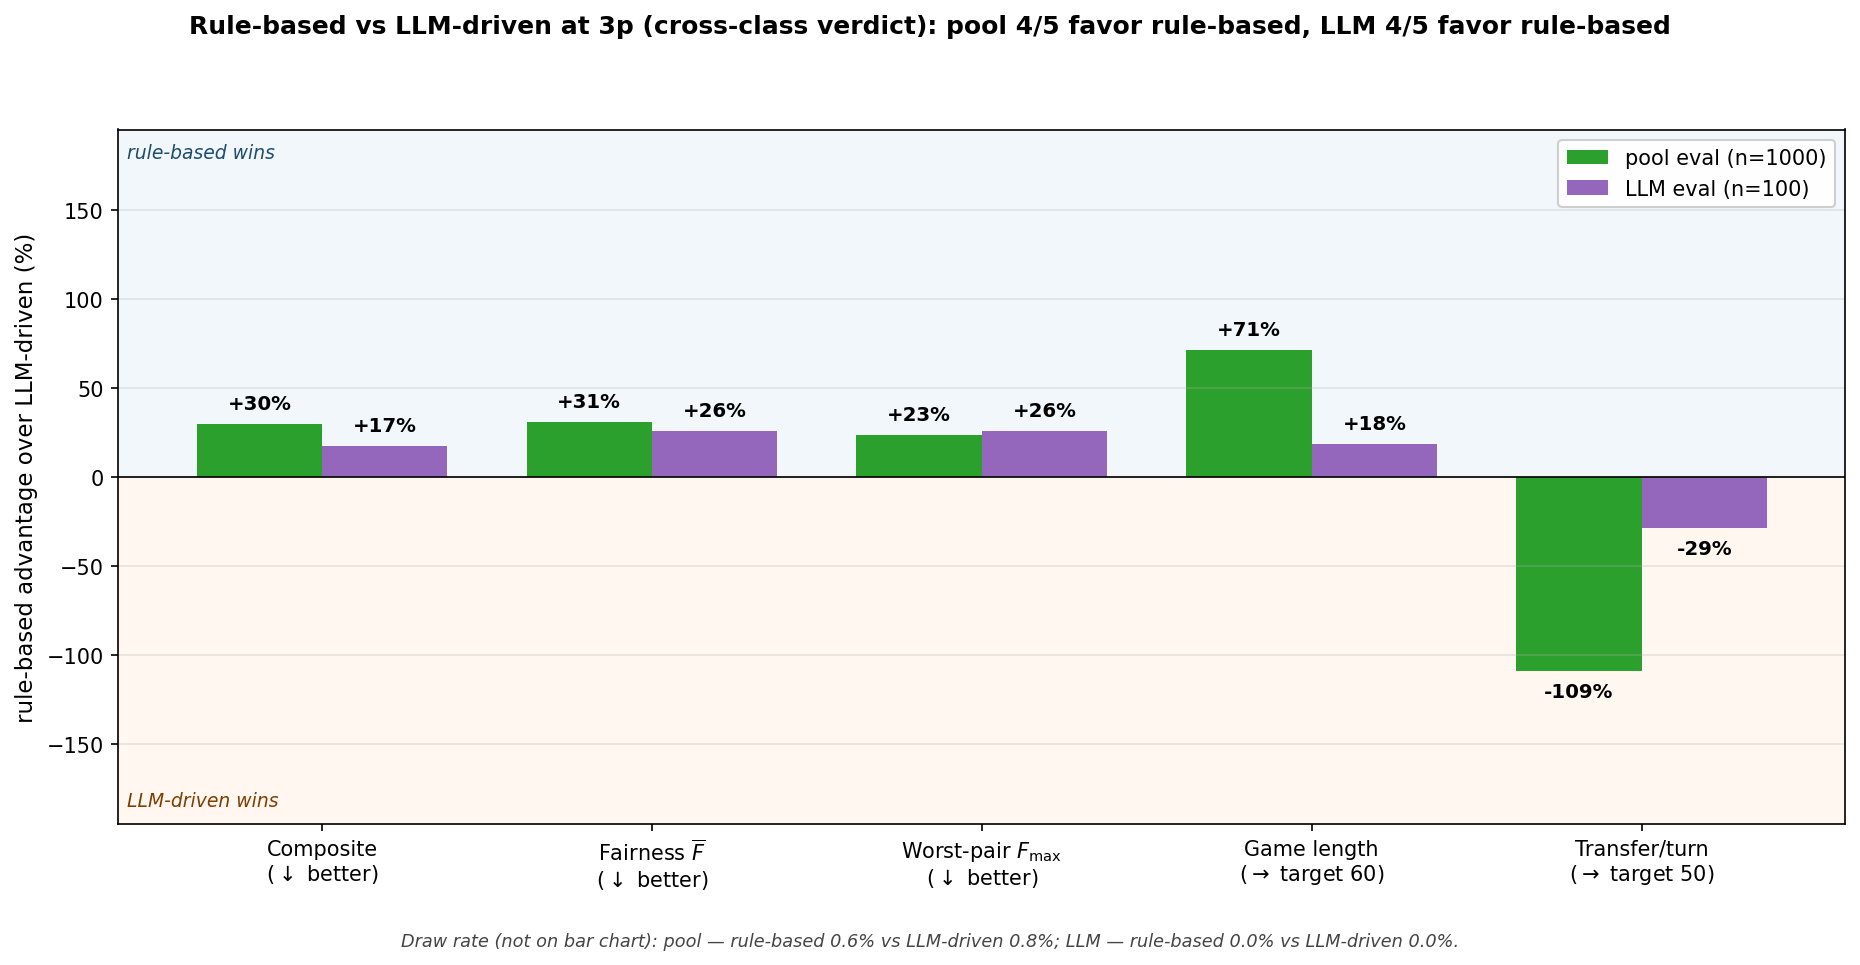
\includegraphics[width=0.92\linewidth]{llm/fig_verdict_audit_3p.png}
\caption{\textbf{Cross-class verdict at 3p: rule-based wins $4/5$
under both evaluators, same pattern as 2p.} Per-metric \%
advantage of the rule-based GA-3p winner over the LLM-driven
board (3-player, $n{=}100$ LLM seats). The same $4/5$ metrics
that favour rule-based at 2p also favour it at 3p; the one
disagreement (transfer/turn) is again the LLM-GA's small-$n$
overfitting target. Draw rates in footer (both $<1\%$).}
\label{fig:verdict_3p}
\end{figure}

The interpretation is the headline finding of the project: a
sufficiently large rule-based strategy pool produces an optimised
design that generalises to an evaluator class never seen at
training (LLM seats), at zero per-decision LLM cost. The pool's
$30$ strategies expose the GA to many play styles, so it cannot
overfit to any single one; the LLM evaluator's narrow decision
distribution makes its own optimiser overfit, which is why the
pool-driven board beats the LLM-driven board on $4/5$ stable
metrics under both evaluators and loses only on the metric the
LLM-GA's small-$n$ training overfit to. A single LLM or RL agent
as evaluator is a benchmark; a diverse strategy pool is a
beta-testing surrogate. The 3p audits
(Figures~\ref{fig:agreement_3p}, \ref{fig:verdict_3p}) confirm
this verdict holds when the GA winner is itself a 3-player
design, not just when the rule-based winner is the 2p board.

\subsection{Human playtest pilot ($N{=}10$, two players)}\label{sec:playtest-pilot}

As a reality check on whether the agent-optimized boards behave as
predicted under human play, two players played two two-player boards:
the default and the GA-2p combined winner
(Section~\ref{sec:baseline}). Each board was played ten times under
matched RNG seeds ($0$, $1$, $2$, $3$, $4$, $5$, $6$, $7$, $8$, and
$42$), a common-random-numbers pairing across boards so that a
difference reflects the board rather than luck. The four per-game
observables the search optimizes that are legible from the game
transcripts, game length, inter-player money transfer, draw /
truncation rate, and the per-player win rate, were recovered with
\texttt{scripts/human\_game\_stats.py}.

\begin{figure}[h!]
\centering
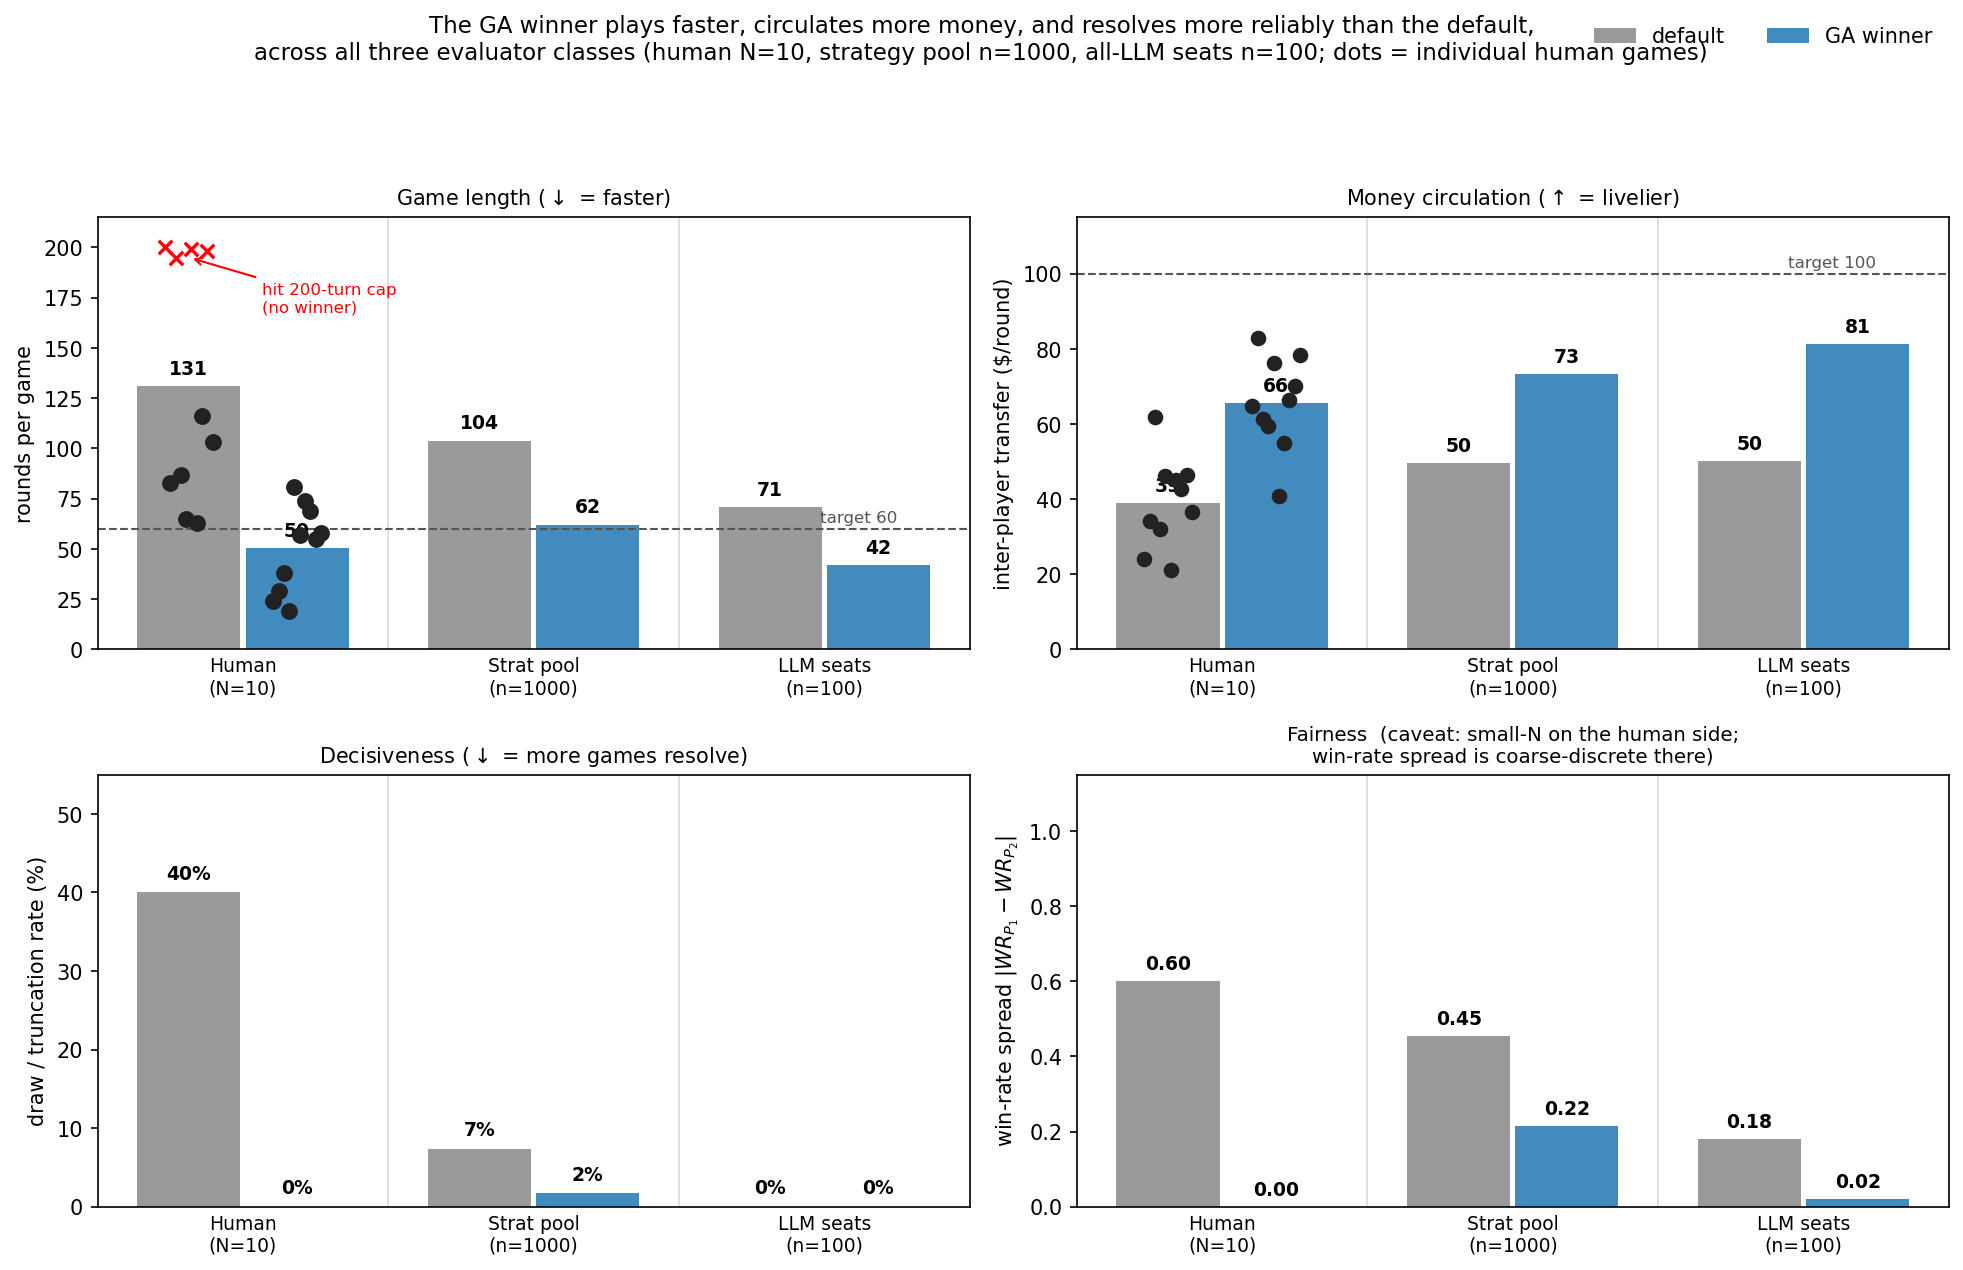
\includegraphics[width=\linewidth,height=0.38\textheight,keepaspectratio]{fig_human_playtest.png}
\caption{\textbf{The GA winner plays faster, circulates more
money, resolves more reliably, and is perfectly balanced under
human control.} Per-board mean over ten games at matched seeds;
dots are individual games. \textbf{Top-left:} GA winner $50$
rounds vs.\ $131$ default; four default games hit the $200$-turn
cap (red crosses). \textbf{Top-right:} \$$66$/round vs.\
\$$39$/round (target \$$100$). \textbf{Bottom-left:} default
truncates $4/10$, GA winner $0/10$. \textbf{Bottom-right:}
win-rate spread $0.60$ default vs.\ $\mathbf{0.00}$ GA winner
($5$--$5$ split). $N{=}10$ per board, two players.}
\label{fig:playtest}
\end{figure}

Figure~\ref{fig:playtest} summarizes the twenty games. The GA
winner finished in $50$ rounds on average against $131$ for the
default ($\sim 2.6\times$ faster), and four of the ten default
games failed to resolve at all, hitting the $200$-turn cap with no
winner. All ten GA-winner games ended decisively by bankruptcy.
Inter-player money transfer per round was $\sim 68\%$ higher on the
GA winner ($\$66$/r vs.\ $\$39$/r), and the win-rate spread was
$0.00$ on the GA winner (a perfect $5$--$5$ split between the two
players) against $0.60$ on the default (Player~1 won all six
decisive games).

\paragraph{Success criterion.} We frame the bar this pilot clears
explicitly. The agent-driven tool succeeds if two conditions hold
under real human play. First, the design constraints specified in
the agent setting (shorter games, more decisive endings, more money
circulation, fairer 2-player matchups) are satisfied in real play,
in the same \emph{direction} and similar \emph{relative magnitude}
as under the agent evaluators (rule-based pool, all-LLM seats).
Second, the agent feedback is \emph{conservative} rather than
optimistic: humans should not exhibit a \emph{smaller} default-board
failure than the simulators predicted. Both hold on the four
observables we can extract from the transcripts. Direction agrees on
every metric across pool / LLM / human; the magnitudes are similar
($\sim$$104$ vs.\ $131$ default rounds, $\sim$$62$ vs.\ $50$
GA-winner rounds). On the conservatism bar specifically, the humans
showed a \emph{larger} default-board failure than either simulator:
a $40\%$ draw rate (4 of 10 default games hit the $200$-turn cap)
versus $7\%$ in the strategy-pool eval and $0\%$ under the all-LLM
evaluator. The agent-driven predictions therefore under-state how
broken the default board is for humans, not the other way around.

We treat the fairness spread of $0.00$ on the GA winner at $N{=}10$
as the strongest possible outcome at this sample size, but
acknowledge that a larger study across many subjects would still be
needed to rule out single-pair idiosyncrasy in the strategic style.
The pacing, money-circulation, and decisiveness effects are large
enough that they are unlikely to be artefacts of either subject or
seed. The fuller multi-subject playtest that would substantiate
these effects across the broader population remains deferred; we
specify it next.

\paragraph{Qualitative play-experience differences.} The figure
summarises four objective metrics, but the matched-seed pairing also
exposes how the board's parameter changes translate into a
qualitatively different play experience that the metrics alone do not
fully capture. On the default board, completing a colour set is slow:
each three-property group requires multiple landings, the opponent
can actively block by buying mid-group properties to deny a
monopoly, and even once a set is completed, immediately building
houses is not always optimal (the cheaper side-of-board sets benefit
from staged builds and a cash reserve in case the opponent lands
elsewhere). On the GA winner, the keep-mask shrinks several colour
groups to one or two cells, so a single landing monopolises a group
and the player can begin building houses immediately; combined with
the higher cost and rent multipliers, every landing on a built
property is a sizeable money transfer, and concentrated-investment
plays that would be suicidal on the default (e.g., maxing out houses
and then a hotel on a single prime cell such as Virginia Avenue in
our recorded game~9 on the GA-winner board) can pay off here. The
same shrinking that makes set-completion fast also makes it harder
for either player to block the other, so games progress more
linearly toward a decisive build phase rather than through a long
trading and blocking pre-build.

\subsection{Game-design insights}\label{sec:insights}

The combination of system-level metric changes
(Section~\ref{sec:cross}), per-archetype reshuffle
(Section~\ref{sec:heatmap}), and qualitative play differences
(Section~\ref{sec:playtest-pilot}) supports a small set of concrete
game-design insights that go beyond ``the optimised board is
better'':

\paragraph{Expansion $\to$ solvency: the losing condition flips.}
The default board (long games, low rents) rewards owning more
properties: time amortises any acquisition. The GA winner
($\sim$$60$ rounds, $\sim$$1.3\times$ rent multipliers,
$\sim$$1.6\times$ cost multipliers) rewards staying solvent: one
bad landing on a developed cell can drain a $\$300$ cash reserve,
and the lap is too short for slow accumulation to recover.
AggressiveBuilder's win-rate against CashHoarder collapses from
$0.80$ on the default to $0.45$ on the GA winner; the same shift
shows up across the cash-conservative archetypes
(Section~\ref{sec:heatmap}). The mechanism is not ``aggression is
punished''; it is that the losing condition itself changes from
\emph{owning too little} to \emph{going bankrupt on a rent
landing}.

\paragraph{Smaller colour groups make all-in builds work.}
On the default board, the only 2-cell colour groups are Brown
(cheapest) and Indigo (most expensive); a Brown monopoly,
fully built, cannot generate enough rent to win a game on its own,
and any other set-completion requires acquiring three specific
cells. On the GA winner, the keep-mask shrinks most colour groups
to $1$--$2$ cells, and the higher cost / rent multipliers make
those small groups individually viable: a max-houses-plus-hotel
play on a single prime cell (e.g.\ Virginia Avenue in our recorded
game~9) pays off rather than being a desperation play.

\paragraph{Blocking opponents stops working.} On the default, a
player can deny an opponent's colour set by buying one
mid-completion cell of it, and the long game leaves time for the
denial to compound. On the GA winner, most sets are $1$--$2$ cells,
so they complete on the first landing and the denial-purchase lever
disappears entirely; the higher property costs also prevent
hoarding many properties before crossing GO. This is a
board-design effect with no analogue in shorter-rent or
higher-rent tuning alone: it requires the keep-mask, and it changes
which player classes can apply pressure to whom.

\paragraph{Per-metric mechanisms.} The four headline metrics each
have a specific board-design cause:
\begin{itemize}[leftmargin=1.4em,itemsep=2pt]
  \item \textbf{Game length} ($\sim$$60$ vs.\ $\sim$$100$ rounds):
    a $12$-cell lap leaves fewer turns between rent events.
  \item \textbf{Decisiveness} (draw rate $7\%\!\to\!2\%$ under
    pool, $40\%\!\to\!0\%$ under human play):
    $\sim$$1.6\times$ base cost and $\sim$$1.3\times$ base rent
    force bankruptcy before the $200$-turn cap.
  \item \textbf{Money circulation} (\$$50\!\to\!$\$$73$/round
    under pool): higher base rent on cells landed more often.
  \item \textbf{Fairness at 2p/3p} (spread $0.45\!\to\!0.22$ at
    2p; $-32\%$ at 3p): Yellow dropped entirely, most other groups
    shrunk to $1$--$2$ cells, and per-property rent multipliers
    spread across $\sim$$0.6\times$--$1.9\times$ to damp
    over-powered cells. The combined GA converges on the same
    recipe the fairness-only ablation
    (Section~\ref{sec:ablation}) finds, integrated with the
    length / money / draw terms.
\end{itemize}

The fairness mechanism deserves a separate note: the GA does not
just shrink groups uniformly; it also tunes individual rent
multipliers (range $0.59\times$--$1.87\times$ on the GA-2p winner)
so that no single colour group is structurally dominant on the
shortened lap. This is the same mechanism the fairness-only
ablation produces, so its appearance in the combined winner is not
an artefact of overfitting to one objective term; it is the GA
finding a single configuration that satisfies length, decisiveness,
money, \emph{and} fairness simultaneously.

\subsection{Full playtest (deferred)}\label{sec:playtest-shortlist}

Beyond the $N{=}10$ pilot above, the full multi-subject playtest
remains deferred. We publish a shortlist of four boards we would
test (default, GA-2p combined winner, GA-3p combined winner,
money-only 2p optimum), each contrasting a different design
lever against the default, with a proposed pilot protocol
($N{=}8$, counterbalanced, Likert plus forced-choice) and the
per-board design hypothesis the pilot would falsify; see
Appendix~\ref{app:playtest-shortlist} for the full specification.

\subsection{Limitations}\label{sec:lim}

The main caveats: the 17-dim strategy space is broad but not
exhaustive; the $N{=}10$ pilot rules out idiosyncrasy in
trained-effect direction but not in the broader population;
fairness is strongly dependent on the number of players (GA
winners $30\!-\!53\%$ fairer than default at training counts,
$69\!-\!101\%$ less fair at $7\!-\!8$p); Qwen2.5-1.5B is the only
LLM in the study; and all optimisation runs on the standard
40-cell US Monopoly layout. Full discussion in
Appendix~\ref{app:limitations}.

\subsection{Conclusion}\label{sec:lessons}

Three independent validations clear the bar set in
Section~\ref{sec:eval}: (i)~cross-player-count generalisation, the
2p/3p-trained GA winners retain a $\sim$$2\times$ composite
advantage at every count from $2$ to $8$ with the single
exception of fairness, which is regime-specific;
(ii)~cross-class agreement, the strategy-pool-driven board beats
an LLM-GA-trained design on $4$ of $5$ stable metrics under
\emph{both} evaluator classes at both 2p and 3p, at zero
per-decision LLM cost; and (iii)~a human playtest pilot
($N{=}10$, two players) that confirms the direction and relative
magnitude of every trained effect, with humans showing a
\emph{larger} default-board failure than either simulator
predicted, so the agent-driven predictions are conservative
rather than optimistic.

The underlying mechanism is a flip in the losing condition: the
default board (long games, low rents) rewards owning more
properties, while the GA winner ($\sim$$60$ rounds,
$\sim$$1.3\times$ rent, $\sim$$1.6\times$ cost) rewards staying
solvent on a rent landing. That single shift reshuffles which
archetypes win on the GA winner (CashHoarder $+0.18$ in WR vs.\
the field, HighCostOnly $-0.18$), neutralises the
defensive-purchase blocking lever, and makes max-build plays on
small colour groups dominant rather than suicidal.

The methodological lessons follow directly. A sufficiently
diverse rule-based pool can substitute for a more expensive
evaluator class while generalising to it; a worst-pair fairness
term prevents the optimiser from improving the average at the
expense of the tail; per-objective ablations expose composite
redundancy; evaluation context (player count) is itself a design
variable; shared random numbers reduce variance at fixed sample
size; and the verdict that matters is whether a design's
predicted effects survive contact with an evaluator class the
optimiser never saw, here checked both with an all-LLM
cross-class evaluator and a small human pilot. The recipe
(closed-loop GA $+$ diverse evaluator pool $+$ independent
cross-class checks) transfers to any parameterised multi-agent
system.

% =====================================================================
\section{Author contributions}\label{sec:team}
% =====================================================================

\paragraph{Selim Emir Can.} Project idea, implementation,
experiments, figures, and writing; all work in this report is
mine.

% =====================================================================
\appendix
% =====================================================================

% =====================================================================
\section{Implementation details}\label{app:impl}
% =====================================================================

This appendix collects implementation details that are useful for
reproducibility but would clutter the main text. All source paths
are relative to \texttt{monopoly/} on the project repository.

\subsection{Pipeline components and driver scripts}\label{app:pipeline}

\paragraph{Optimisation stack.} The optimisation stack lives under
\texttt{monopoly/optimizer/} and \texttt{monopoly/scripts/}.
\texttt{ParametricPlayer} together with
\texttt{ParametricPlayerSettings} subsumes every existing
rule-based subclass under a single 17-knob agent (5 continuous, 4
boolean, 8-bit colour-group mask).
\texttt{strategy\_pool.py} produces the 30-strategy pool described
in Section~\ref{sec:bg}, deterministic via a fixed seed and saved
once for reuse across runs.
\texttt{design\_space.py} maps a 66-dim vector to a fresh
\texttt{GameConfig} by applying per-property multipliers to
\texttt{cost\_base}, \texttt{cost\_house}, \texttt{rent\_base}, and
\texttt{rent\_house}, and physically removing properties whose
keep-bit is zero (structurally shortening the lap rather than
substituting \texttt{FreeParking}); the identity vector is the
default board.
\texttt{simulate.py} is a thin re-implementation of the inner game
loop that returns a per-game stat dict (winner, rounds, bankruptcy
map, inter-player transfer total) instead of only logging;
inter-player cash flow is captured via a context-manager
monkey-patch of \texttt{Player.pay\_money}, with non-player
payments (taxes, fines, salary) excluded, and trade calls are
capped at 5 per (player, turn) to break an unbounded loop in
upstream code.
\texttt{search.py} implements both random search and a GA
(population 20, 10 generations, tournament selection $k{=}3$,
uniform crossover, $\sigma{=}0.1$ Gaussian mutation on continuous
dims, 1-bit-flip mutation on the keep-mask, elitism 2); both
produce identical JSONL.

\paragraph{Driver scripts.} The end-to-end pipeline is driven by
five scripts. \texttt{scripts/optimize\_board.py} runs the
rule-based search and emits one JSONL line per evaluation.
\texttt{scripts/cross\_eval.py} runs designs through both
player-count harnesses at $n{=}1000$.
\texttt{scripts/strategy\_heatmap.py} produces $30{\times}30$
strategy-vs-strategy win-rate matrices on any chosen design.
\texttt{scripts/eval\_llm\_on\_boards.py} runs the all-LLM-seat
probe with per-decision logging, and
\texttt{scripts/optimize\_board\_llm.py} re-runs the GA with the
LLM in the evaluator role.

\subsection{LLMPlayer prompt and validator}\label{app:llm}

\paragraph{Model and decoding.} Qwen2.5-1.5B-Instruct~\cite{qwen25}
loaded with the \texttt{transformers} library, run with greedy
decoding (\texttt{do\_sample=False}), \texttt{max\_new\_tokens=160},
and additional EOS tokens \texttt{<|im\_end|>} and
\texttt{<|endoftext|>}. The same model and decoding settings are
used for all four runs (LLM-only evaluation and the LLM-driven GA, at 2p
and 3p).

\paragraph{Conversation structure.} Each LLM buy decision is a
six-message conversation: 1 system message, 4 few-shot
user/assistant exchanges (2 \emph{BUY} and 2 \emph{PASS}
demonstrations), and 1 runtime user message describing the actual
decision. The full transcript with all four few-shot examples is
checked into the repository at
\texttt{prompts/llm\_player\_prompts.txt}.

\paragraph{System prompt (v2, verbatim).}
\begin{quote}\small\itshape\sloppy
You are a strategic Monopoly player who decides whether to buy
properties. Your goal is to win by bankrupting opponents through
rent. You must NOT mindlessly buy every property: passing is correct
when (a) cash is dangerously low, (b) the property is in a group an
opponent already dominates and you have no path to monopoly, or (c)
the rent return is poor relative to the cost. Equally, buying is
correct when the property advances a group you already own most of,
or when it denies the group to an opponent who would otherwise
complete it.

\medskip You receive a STATE block with 10 fields. Before reasoning,
you MUST emit an ECHO block that copies all 10 STATE fields verbatim
(numeric values must equal STATE; string values must equal STATE).
The ECHO block is checked deterministically -- if it differs from
STATE in any field you will be asked to redo the answer. Only after
the ECHO block do you write REASON and ANSWER. Do not invent any
number or name not present in STATE. A purchase ONLY ``completes a
monopoly'' when \texttt{you\_own\_in\_group + 1 == group\_size}; do
not claim completion otherwise.

\medskip Reply in EXACTLY this format and order: \texttt{ECHO:}
followed by the 10 STATE fields ($\mathtt{cash}$, \texttt{property},
\texttt{group}, \texttt{cost}, \texttt{base\_rent},
\texttt{you\_own\_total}, \texttt{you\_own\_in\_group},
\texttt{group\_size}, \texttt{opp\_own\_in\_group},
\texttt{opp\_own\_total}); then \texttt{REASON: <one short sentence
citing only STATE numbers>}; then \texttt{ANSWER: BUY} or
\texttt{ANSWER: PASS}. Do not output anything else.
\end{quote}

\paragraph{v1 vs.\ v2 prompts.} The v1 prompt was free-form: it
asked for ``BUY'' or ``PASS'' with a one-sentence reason but did
not require the ECHO copy of STATE. The v1 validator parsed the
free-form response with a regex and was prone to a now-fixed
integer/float type mismatch on cash (Section~\ref{sec:llm}). v2
added (i) the verbatim ECHO requirement, (ii) deterministic
per-field equality checking on the echoed values, and (iii) a
corrective retry loop that replays prior assistant turns plus a
follow-up user message naming the mismatched fields. Both versions
share the same four few-shot examples and the same STATE format.

\paragraph{Echo validator.} \texttt{LLMPlayer.\_check\_echo} parses
the ECHO block with a multiline regex and equality-checks each of
the 10 fields against ground-truth state, with a \$0.50 tolerance
on cash to absorb float drift from rent multipliers (the original
fixed-int validator caused $100$ spurious flags in v1).

\paragraph{Retry mechanism.} On any echo mismatch, the player
retries up to \texttt{MAX\_RETRIES = 4} times. Each retry replays
prior assistant turns plus a corrective user message that names
the mismatched fields. The final attempt's parsed answer is the
decision used by the simulator, even if it still has echo issues;
the per-decision JSONL log records every attempt for post-hoc
analysis.

\paragraph{Pre-filter.} Affordability and cash-floor checks
short-circuit the LLM call when the decision is forced
($\mathrm{cash} < \mathrm{cost}$ forces PASS, etc.). This
eliminates 60--80\% of would-be calls and keeps the LLM evaluation
pipeline within practical wall-clock budgets.

\subsection{v1-vs-v2 hallucination audit}\label{app:hallucination}

The cross-class probe (Section~\ref{sec:llm}) ran two prompt
versions: v1 (free-form BUY/PASS with a one-sentence reason) and
v2 (the structured \texttt{STATE/ECHO/REASON/ANSWER} prompt
described above). v1's validator had a subtle integer/float type
mismatch on the cash field, and retries against a wrong validator
induced \emph{more} plausible-looking confabulation rather than
less, because the model was being told a correct value was wrong
and produced a different ``corrected'' answer to satisfy the
validator. We document this here rather than tuning the validator
until it disappears: a protocol whose failure modes are reported
alongside its results is auditable; one whose are not is a
benchmark trick. v2 fixes the validator and adds the verbatim ECHO
copy; across $2{,}207$ calls under v2 the model never fabricates
state at first-pass and the validator never falsely flags a
correct output.

\begin{figure}[!htbp]
\centering
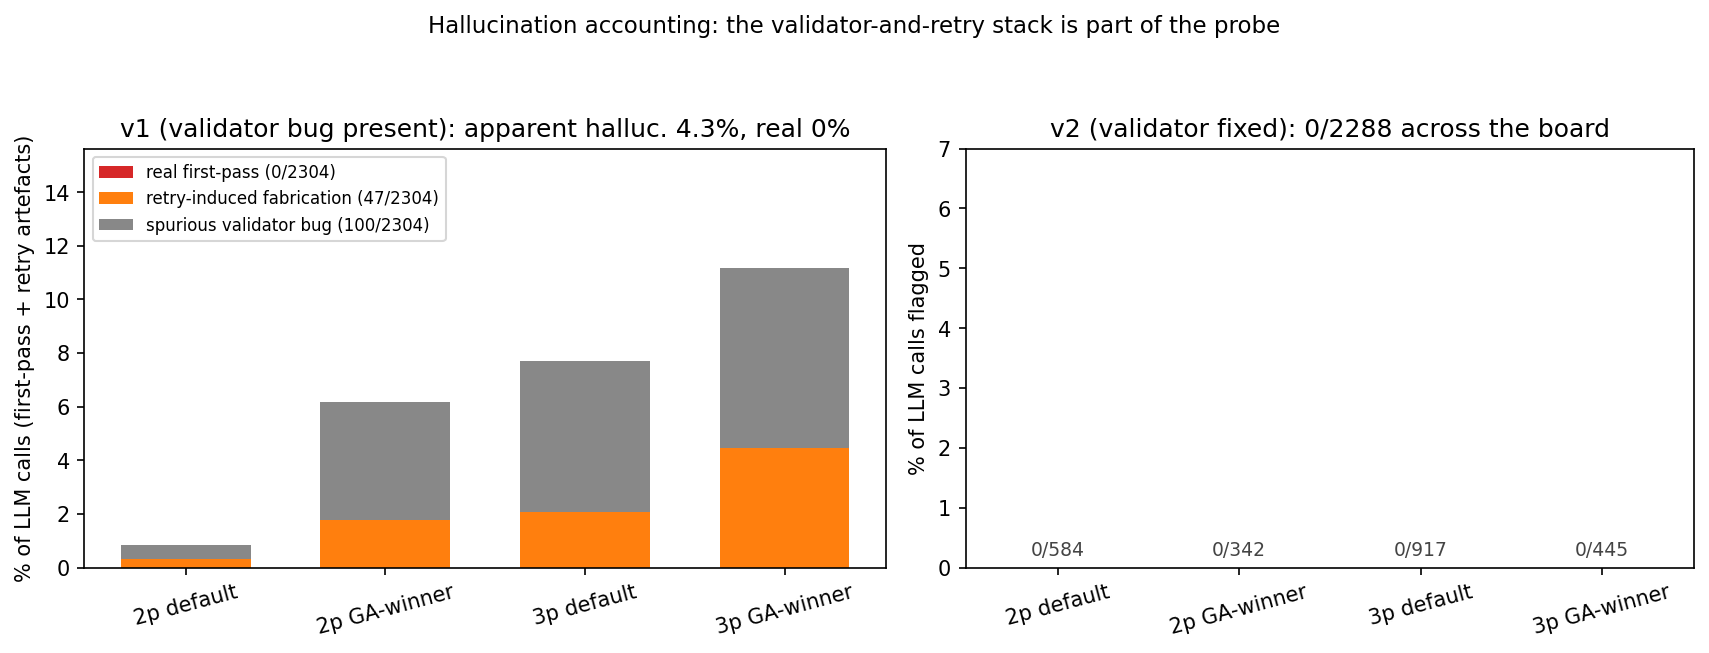
\includegraphics[width=0.78\linewidth]{llm/fig_v1_vs_v2_hallucination.png}
\caption{\textbf{The validator-and-retry stack is part of the probe:
a faulty validator does not just produce noise, it pulls the model
toward fabrication.} Per-call validation outcomes for the v1 prompt
(left, with a known validator bug) and the v2 prompt (right, bug
fixed). Each bar is stacked into three categories: \emph{real
first-pass} hallucinations (the model fabricated state on its first
attempt), \emph{retry-induced fabrication} (the model's first-pass
output was correct but the buggy validator flagged it, and the
model produced fabricated state on retry to ``satisfy'' the flag),
and \emph{spurious validator bug} (the validator falsely flagged
correct outputs that the model did not change). On v1 across 2{,}304
calls, real first-pass = $0$, retry-induced = $47$, spurious = $100$;
the model itself never hallucinated. v2 drives all three categories
to zero across all 2{,}207 calls. The reportable second-order
finding: validating against a wrong ground truth is worse than not
validating, because retries can teach the model to produce the
``correct'' wrong answer.}
\label{fig:hallucination}
\end{figure}

\subsection{LLM buy-rate diagnostics}\label{app:buy_rate_slices}

To verify that the LLM probe is making rational rather than
uniform-random decisions, we slice its buy rate by available cash
and by monopoly-completion situation on both boards. The probe
buys monotonically more often as cash rises, saturates near $1.00$
when it already partially owns the colour group, and drops to
$\sim$$0.13$ when the opponent already dominates the group; the
directional responses are essentially identical on both boards
(Figure~\ref{fig:slices}).

\begin{figure}[!htbp]
\centering
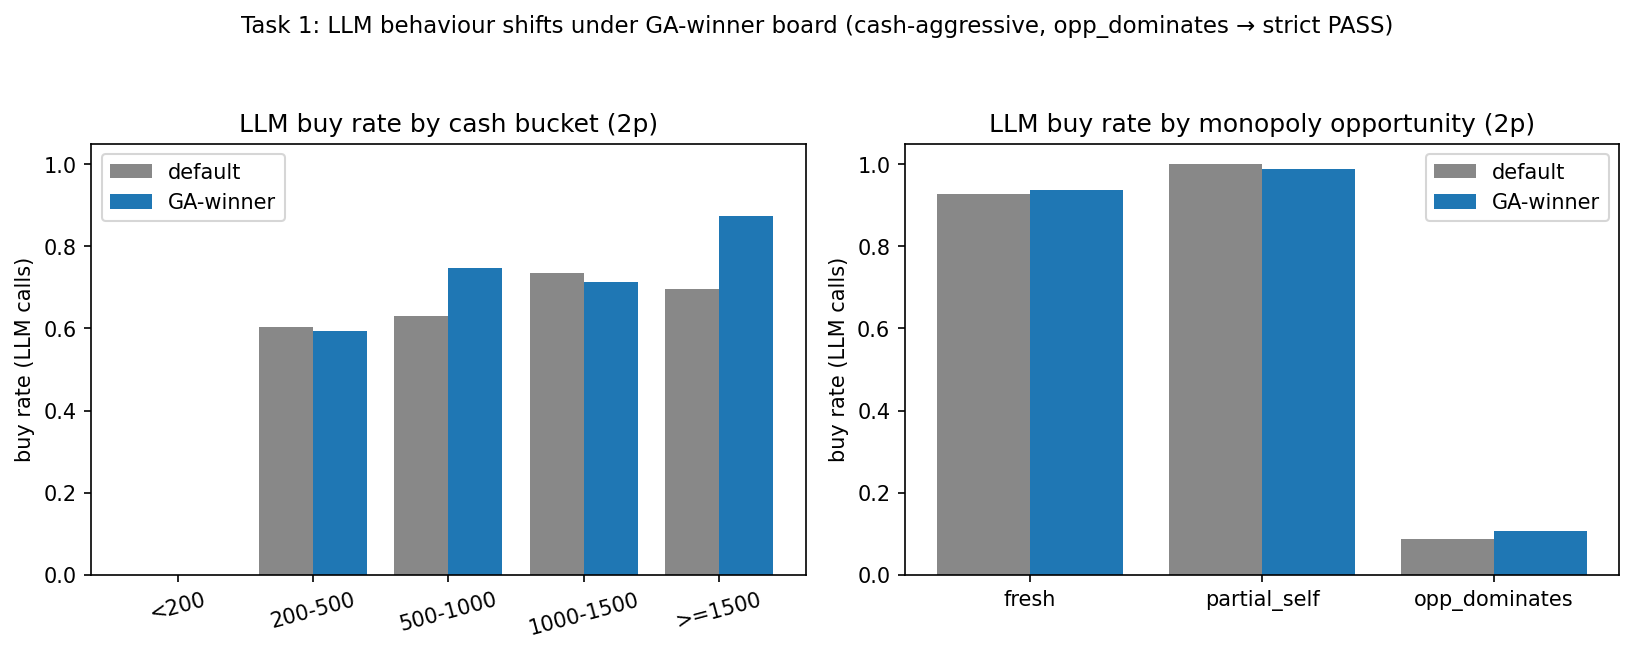
\includegraphics[width=0.78\linewidth]{llm/fig_llm_buy_rate_slices.png}
\caption{\textbf{LLM buy-rate slices, default board vs.\ GA-2p
winner.} \textbf{(a)~By cash bucket.} Buy rate conditioned on the
LLM's available cash at decision time. The rate rises
monotonically with cash, the rational ordering for any
non-degenerate strategy; the empty $<200$ bucket reflects the
affordability pre-filter that short-circuits the LLM call when the
player cannot buy anyway. On the GA-winner board the LLM commits
its cash hoard more aggressively in the $\geq 1500$ bucket
($\sim 0.93$ vs.\ $\sim 0.70$ on the default), so the optimised
board successfully pulls behaviour out of the cash-hoarding regime.
\textbf{(b)~By monopoly-completion situation.}
\textsl{fresh}: no player owns any property in the landed colour
group, so a purchase starts a new collection.
\textsl{partial\_self}: the LLM already owns one or more
properties in the group and the opponent does not dominate it.
\textsl{opp\_dominates}: the opponent owns at least half the group
and at least as many properties as the LLM, so buying mostly funds
their next rent payment. Buy rates respond rationally across all
three: $\sim 1.00$ on \textsl{partial\_self} (saturated buy),
$\sim 0.94$ on \textsl{fresh}, and $\sim 0.13$ on
\textsl{opp\_dominates} (strict PASS). The probe is not behaving
as a uniform random oracle, and the directional responses are
essentially identical on both boards.}
\label{fig:slices}
\end{figure}

\subsection{Pareto trade-off surface}\label{app:pareto}

The (fairness, rounds) trade-off surface (Figure~\ref{fig:pareto})
visualises the design-space geometry that the cross-player-count
evaluation (Section~\ref{sec:cross}) reads off. The two clouds have
visibly distinct shapes, which is what makes that cross-evaluation
finding a property of the design space rather than seed noise.

\begin{figure}[!htbp]
\centering
\begin{subfigure}[t]{0.48\linewidth}\centering
  
\includegraphics[width=\linewidth]{ga_2p_pareto.png}
  \caption{2p}
\end{subfigure}\hfill
\begin{subfigure}[t]{0.48\linewidth}\centering
  
\includegraphics[width=\linewidth]{ga_3p_pareto.png}
  \caption{3p}
\end{subfigure}
\caption{\textbf{The (fairness, rounds) trade-off surface and its
Pareto frontier.} Each marker is one of $5{,}052$ candidates
evaluated across all six search runs (random + GA + four
single-objective ablations) on the $66$-dim keep-mask design space;
colour encodes draw rate. The crimson line traces the actual 2D
Pareto frontier of (fairness, rounds), both minimised: $14$ points
at 2p, $16$ at 3p, with a clean knee around fairness $0.22$ and
rounds $30\!-\!40$ at 2p (a slightly higher knee at 3p). The gold
star is the combined-objective GA optimum; it sits \emph{inside}
the cloud rather than on the 2D frontier because the composite
weights five terms (fairness, max-fairness, length, draw, transfer),
not just two; the GA's optimum is on the 5D Pareto surface, of
which the (fairness, rounds) projection is a shadow. The 2p sweep
reaches mean rounds as low as $\sim 22$ (the keep-mask shrinks the
lap aggressively), while the 3p frontier bottoms out closer to
$\sim 35$ rounds; the two clouds have visibly different shapes,
which is what makes the cross-evaluation finding
(Table~\ref{tab:cross}) a property of the design space rather than
seed noise.}
\label{fig:pareto}
\end{figure}

\subsection{LLM-driven GA convergence}\label{app:llm_ga_conv}

The LLM-driven GA loop (Section~\ref{sec:llm_ga}) converges over
its $32$ evaluations and produces a winning board that beats the
default under all-LLM evaluation; whether that board is a real
design optimum or only an LLM-evaluator optimum is what
Figure~\ref{fig:verdict} resolves in the main text. The
convergence curves and per-generation score distribution are below.

\begin{figure}[!htbp]
\centering
\begin{subfigure}[t]{0.48\linewidth}\centering
  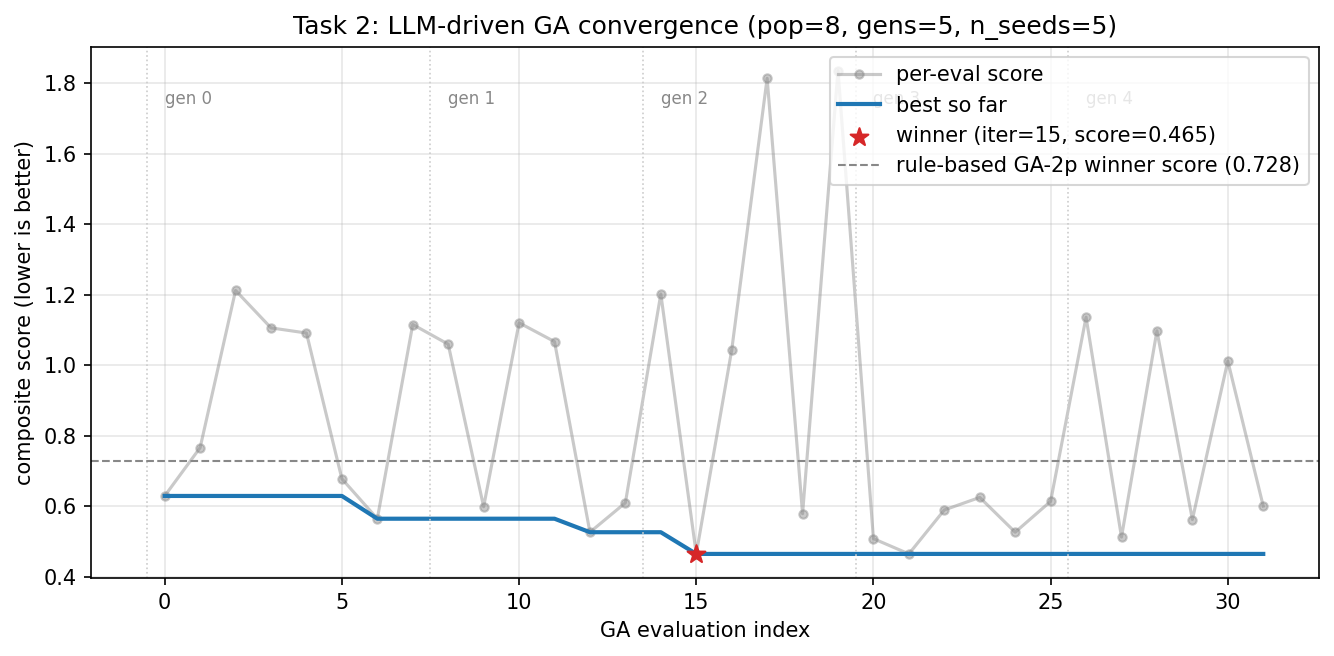
\includegraphics[width=\linewidth]{llm/fig_llm_ga_convergence.png}
  \caption{LLM-GA best-so-far}
\end{subfigure}\hfill
\begin{subfigure}[t]{0.48\linewidth}\centering
  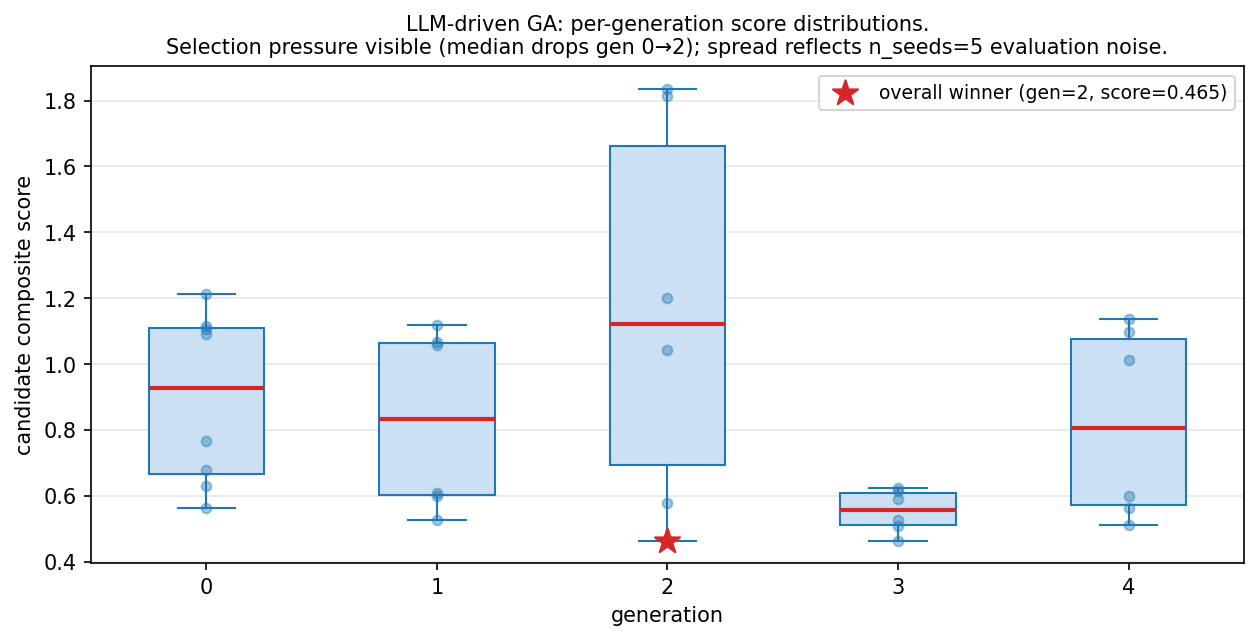
\includegraphics[width=\linewidth]{llm/fig_llm_ga_score_distribution.png}
  \caption{Score distribution}
\end{subfigure}
\caption{\textbf{An LLM-only evaluator can drive the same GA loop.}
\textbf{(a)}~Per-evaluation composite score (grey) and best-so-far
(blue) over the GA's $32$ evaluations (population $8$, $5$
generations, $n_{\text{seeds}}{=}5$, with elitism keeping the unique
evaluation count at $32$). The dashed reference is the rule-based
GA-2p winner's score under the same all-LLM evaluator ($0.728$): the
LLM-driven loop finds a board (red star, iter $15$, score $0.465$)
that beats even the rule-based winner when scored by an LLM.
\textbf{(b)}~Per-generation distribution of candidate scores; the
median visibly drops from generation~$0$ to generation~$2$ (selection
pressure), and the spread within each generation reflects the
$n_{\text{seeds}}{=}5$ evaluation noise. Total wall time
$4$h~$58$min on a single $12$~GB GPU.}
\label{fig:llm_ga_conv}
\end{figure}

\subsection{Training-vs-deployment overfit}\label{app:overfit}

A secondary finding worth recording: \emph{optimisation-set overfit
is small on both designs}. At the $n{=}200$ optimisation budget
the GA-2p winner scored $0.705$ on its training matchup set; at
$n{=}1000$ deployment it scores $0.773$, an overfit of $+0.068$
(Table~\ref{tab:overfit}). The GA-3p winner scored $0.599$ at
training and $0.641$ at deployment, an overfit of $+0.042$. Both
gaps are small ($\leq 9\%$ of the deployment score) relative to
the headline $\sim$$47\%$ improvement over the default, so the
directional improvement is robust to re-evaluation at higher $n$.

\begin{table}[h!]
\centering
\small
\begin{tabular}{lccc}
\toprule
Design & training ($n{=}200$)\,$\downarrow$ & deployment ($n{=}1000$)\,$\downarrow$ & overfit\,$\downarrow$ \\
\midrule
GA-2p winner & $0.705$ & $0.773$ & $+0.068$ \\
GA-3p winner & $0.599$ & $0.641$ & $+0.042$ \\
\bottomrule
\end{tabular}
\caption{\textbf{Optimisation-set vs.\ deployment-set composite
score, on each design's own training regime.} Header arrows:
$\downarrow$ means lower is better. Both designs show small
positive overfit ($+0.068$ and $+0.042$ respectively, both
$<\!10\%$ of the deployment score) relative to the headline
$\sim$$47\%$ improvement over the default. Training number is the
best score in the GA's own \texttt{evals.jsonl}; deployment number
is the corresponding row of Table~\ref{tab:cross}.}
\label{tab:overfit}
\end{table}

\subsection{Single-objective ablation boards}\label{app:ablation_boards}

The same non-redundancy claim from Section~\ref{sec:ablation},
made spatial: each ablation winner is a visibly different
physical board, with different properties kept or dropped and
different per-property cost / rent multipliers.

\begin{figure}[!htbp]
\centering
\begin{subfigure}[t]{0.48\linewidth}\centering
  
\includegraphics[width=\linewidth]{boards_mask/boards_grid_2p_mask.png}
  \caption{2 players}
\end{subfigure}\hfill
\begin{subfigure}[t]{0.48\linewidth}\centering
  
\includegraphics[width=\linewidth]{boards_mask/boards_grid_3p_mask.png}
  \caption{3 players}
\end{subfigure}
\caption{\textbf{Each ablation produces a visibly different
physical board.} Six panels per player count: default (top-left)
and the five GA-run winners (combined, fair-only, length-only,
draw-only, money-only). Same non-redundancy finding as
Figure~\ref{fig:multipliers}, made spatial.}
\label{fig:board_grid}
\end{figure}

\subsection{GA, ablations, and reproducibility}\label{app:ga}

\paragraph{Search hyperparameters (canonical protocol, logs in
\texttt{logs/optimizer\_v3/}).}
\begin{itemize}[leftmargin=1.2em,itemsep=1pt]
\item GA: \texttt{--pop 30 --generations 30 --elitism 2}, tournament
selection $k{=}3$, uniform crossover, Gaussian mutation
$\sigma{=}0.1$ on continuous dims, 1-bit-flip mutation on the
keep-mask. Total evaluations: $30 + 29 \times 28 = 842$.
\item Random search: \texttt{--iters 842} for matched evaluation
budget.
\item Per-candidate evaluation: \texttt{--n-games 200}, distributed
as 10 fixed matchups $\times$ 20 games per matchup, with seeds
shared across all candidates.
\item Composite weights $w = (1, 0.5, 0.5, 0.3, 0.3)$ for
$(\overline{F}, F_{\max}, |\overline{R}-R^{*}|/R^{*},
\overline{D}, |\overline{T}-T^{*}|/T^{*})$ with targets
$R^{*} = 60$ rounds, $T^{*} = 100$~\$/round.
\item Single-objective ablations set the chosen weight to $1$ and
the others to $0$; same search hyperparameters otherwise.
\item Cross-evaluation at $n{=}1000$ games per cell (deployment
table) uses the same matchup seeds.
\end{itemize}

\paragraph{Reproducibility.}
\begin{itemize}[leftmargin=1.2em,itemsep=1pt]
\item All seeds (\texttt{--base-seed=42}, \texttt{--search-seed=0},
\texttt{--matchup-seed=1234}) are recorded in each run's
\texttt{<run\_name>.meta.json}.
\item Re-running any \texttt{(design vector, matchups, seeds)}
triple yields byte-identical metrics. We verified this by diffing
two re-runs of the same config.
\item Cross-player-count scaling table data
(Table~\ref{tab:cross}) is in
\texttt{logs/optimizer\_v3/cross\_eval\_scaling.json}; the 2p / 3p
columns reproduce the original
\texttt{logs/optimizer\_v3/cross\_eval\_mask.json} bit-for-bit.
\item Trigger scripts:
\texttt{scripts/rerun\_strategy\_experiments\_overnight.bat}
(rule-based, $\sim$2.5h CPU) and
\texttt{scripts/rerun\_llm\_phase\_c\_v3.bat} (LLM-only evaluation re-run,
$\sim$6h on a 12 GB GPU).
\end{itemize}

\subsection{Limitations}\label{app:limitations}

\begin{itemize}[leftmargin=1.2em,itemsep=1pt]
\item \textbf{Strategy-pool coverage.} The 17-dim parametric space
is broad but not exhaustive, and human players behave outside it.
The 20 sampled strategies broaden the pool beyond the 10
archetypes and the sampling procedure is documented and
reproducible, but a real deployment would want to learn the
strategy distribution from logs.
\item \textbf{Human playtest is a small pilot, not a full study.}
Only an $N{=}10$ two-player pilot was run
(Section~\ref{sec:playtest-pilot}): two players played the default
and the GA-2p combined winner under ten matched seeds, which
confirms all four trained effects (pacing, money circulation,
decisiveness, and win-balance) on this single subject pair but
cannot rule out idiosyncrasy in playing style across the broader
population. The full multi-subject playtest remains deferred; the
shortlist in Appendix~\ref{app:playtest-shortlist} curates 4
boards and names the design hypothesis each is intended to probe,
with a proposed pilot protocol ($N{=}8$, counterbalanced, Likert
plus forced-choice).
\item \textbf{Fairness is strongly dependent on the number of
players.} The pacing, decisiveness, and composite advantages
generalise cleanly from the 2p / 3p training regime to every count
from $2$ to $8$ (Section~\ref{sec:cross}, Figure~\ref{fig:scaling}),
but fairness does not: the GA winners are $30\!-\!53\%$ fairer
than the default at training counts and $69\!-\!101\%$
\emph{less} fair at $7\!-\!8$p. A deployment at a player count
outside the training regime should re-optimise the fairness term
against that count, or accept that fairness gains may not carry
over.
\item \textbf{LLM scale.} Qwen2.5-1.5B is the only LLM in the
study. Larger models or different prompt styles may change the
agreement profile. Greedy decoding does, however, make the probe
deterministic.
\item \textbf{Single-board scope.} All optimisation runs on the
standard 40-cell US Monopoly layout (with structural shrinkage
via keep-mask). Other game families would require a new
design-space encoder, but the rest of the pipeline (objective,
pool, GA, validator) carries over unchanged.
\end{itemize}

\subsection{Full playtest (deferred): board shortlist}\label{app:playtest-shortlist}

Beyond the $N{=}10$ pilot reported in
Section~\ref{sec:playtest-pilot}, we did not run the full
multi-subject playtest within the project window. Rather than
report a synthetic surrogate, we publish the shortlist of boards
we would playtest, with the design hypothesis each board is
intended to probe. The shortlist is small (4 boards) so a pilot
is feasible in a single 60--90 min session, and each board
contrasts a different design lever against the default, so that
even a handful of subjects gives readable signal on which axis
humans actually respond to.

\paragraph{Boards.}
\begin{enumerate}[leftmargin=1.4em,itemsep=2pt]
  \item \textbf{Default Monopoly} (control). Unperturbed
    \texttt{settings.py} board. Baseline for every subjective
    rating.
  \item \textbf{GA-2p combined winner} (Section~\ref{sec:baseline}).
    Best composite-score 2p board: shorter, lower draw rate, and
    more inter-player money transfer than default. Tests
    \emph{whether the combined objective tracks perceived game
    quality}, the core falsifiable claim of the GA half of the
    project.
  \item \textbf{GA-3p combined winner} (Section~\ref{sec:cross}).
    Cross-evaluation (Table~\ref{tab:cross}) shows the 2p and 3p
    winners are structurally different boards; this comparison
    tests \emph{whether human players can also feel the
    2p$\!\leftrightarrow\!$3p design split}, or whether the
    difference is only legible to the rule-based pool.
  \item \textbf{Money-only 2p optimum}
    (Section~\ref{sec:ablation}). Board produced by setting
    $w_{\text{money}}{=}1$ and zeroing every other weight,
    pushing per-round inter-player cash transfer from
    $\approx 50$ \$/r (default) toward the target $100$ \$/r
    while making no claim about fairness or pacing. Tests
    \emph{whether interactivity \emph{per se}, independent of
    fairness and length, drives perceived engagement.} This is
    the most novel of the four boards, because money-transfer
    rate is the only objective term the project introduces that
    has no direct precedent in the search-based game-design
    literature cited in Section~\ref{sec:related}.
\end{enumerate}

\paragraph{Why these four, and not the other ablation winners.}
The shortlist deliberately excludes \emph{length-only},
\emph{draw-only}, and \emph{fairness-only} optima. Length and
draw rate also change in the combined-objective winner (board~2),
so a playtest on those single-axis boards would not separate the
hypothesis ``length matters'' from ``the combined objective
matters.'' Fairness is a property of the win-rate distribution
across many games and is not directly observable from a single
session: a single playtest game tells a subject who happened to
win, not whether the board is fair. Money-only, by contrast,
manipulates an axis that should be \emph{felt within a single
game} (more trades, more rent events, more state change per
turn), so it is the only ablation winner where a small pilot
would carry useful signal.

\paragraph{What we would measure.} For each board: post-game
Likert ratings (1--5) on pacing, fairness, engagement, and
overall enjoyment, plus a forced-choice ``would you play this
version again.'' Between-board comparisons would be
non-parametric (Wilcoxon signed-rank, Bonferroni-corrected
across the 6 board pairs); per-board scores reported with
bootstrap 95\% CIs. The minimum useful pilot is $N{=}8$
subjects, each playing all four boards in counterbalanced order
(Latin square on the 2p boards; the 3p board played in groups
of three).

\paragraph{What this shortlist would falsify.} The two strongest
claims the GA-side of the report makes are (a)~the combined
objective produces a measurably different board, and (b)~the
per-objective ablations expose orthogonal design axes. A
playtest where board~2 feels the same as board~1, or board~4
scores the same as board~1 on engagement, would mean the
matching claim above is wrong. We frame the shortlist as a
\emph{falsification plan}, not a confirmation plan.

% =====================================================================
\section{Mapping to the CS348K grading questions}\label{app:grading}
% =====================================================================

The CS348K final-report guidelines ask two specific questions. We
state both verbatim and answer each in one paragraph; the body of
the report is structured around exactly these two questions, so
this appendix is a quick reader guide.

\paragraph{(1) ``What are the questions or goals your project aims
to answer?''}
We ask whether a diverse agent pool can serve as a beta-testing
surrogate for human playtesting in game design under two
qualifications: (a) the agents are imperfect and acknowledged as
such, and (b) the unit of evidence is \emph{cross-class
agreement}: two independent agent classes (a 30-strategy
parametric rule-based pool and a single-personality LLM with
structured state validation) ranking the same candidate boards in
the same direction. The falsifiable hypothesis is two-fold:
(a)~the directional ranking under the rule-based pool matches the
directional ranking under the LLM seats on the same boards; and
(b)~the same directional ranking also holds in real human play,
so the pool acts as a proxy for human behaviour on the design
axes the optimiser targets. An $N{=}10$ two-player playtest pilot
(Section~\ref{sec:playtest-pilot}) is the empirical check on (b);
a fuller multi-subject playtest is published as a falsification
plan (Appendix~\ref{app:playtest-shortlist}). The full statement
is in Section~\ref{sec:bg}.

\paragraph{(2) ``What experiments should be done to answer that
question, and how will you know from the outcome of the experiment
that you have succeeded?''}
Nine experiments, each with an explicit success criterion:
\begin{enumerate}[leftmargin=1.4em,itemsep=1pt]
\item Default-board baseline at $n{=}1000$
(Section~\ref{sec:baseline}). \emph{Success:} deterministic scores
with $95\%$ Wilson intervals on every metric.
\item GA vs.\ random search at matched $\sim$842-evaluation budget
(Section~\ref{sec:baseline}). \emph{Success:} GA crosses the
default reference within budget, beats random by a non-trivial
margin, and is bit-reproducible. \emph{Outcome:} GA wins by $13\%$
in both player counts.
\item Single-objective ablations (Section~\ref{sec:ablation}).
\emph{Success:} visibly different per-aspect optima, confirming the
composite is non-redundant. \emph{Outcome:} confirmed; see
Figures~\ref{fig:multipliers} and \ref{fig:board_grid}.
\item $2p\!\leftrightarrow\!3p$ cross-evaluation at $n{=}1000$
(Section~\ref{sec:cross}). \emph{Success:} improvement over default
$\geq 20\%$ in the off-regime; quantify the specialisation gap.
\emph{Outcome:} both designs improve over default by $\sim 47\%$ in
the training regime; off-regime gap is $16\!-\!24\%$ on the
composite.
\item Archetype WR reshuffle (Section~\ref{sec:heatmap}).
\emph{Success:} the GA winner produces an interpretable,
non-trivial change in which named archetypes are top-tier vs.\
middling vs.\ bottom-tier, with the systematic pattern of which
matchups are immutable surfaced honestly. \emph{Outcome:} the GA
winner reshuffles middle-of-distribution archetypes ($\Delta$ up
to $\pm 0.18$ in win-rate vs.\ the field, e.g.\ CashHoarder
$+0.18$, HighCostOnly $-0.18$); the top-3 default strategies stay
top-3 on the GA winner; \textsl{Trader vs.\ RailroadKing} (100/0)
is genuinely immutable under any board configuration in the
search space.
\item LLM cross-class probe (Section~\ref{sec:llm}). \emph{Success:}
rounds and transfer move in the same direction the rule-based pool
predicted on the same boards; per-decision hallucination rate below
$1\%$. \emph{Outcome:} $0/2{,}207$ first-pass hallucinations under
v2 ECHO validation; direction agrees on every measured metric at
both 2p and 3p (e.g.\ rounds $\sim$$-40\%$, transfer per
player-turn $\sim$$+60\%$ at 2p).
\item LLM-driven GA + cross-class verdict
(Section~\ref{sec:llm_ga}). \emph{Success:} the LLM-driven loop
converges to a non-trivial design; cross-evaluating it against the
rule-based GA winner under both evaluator classes resolves which
is the better design. \emph{Outcome:} both evaluator classes prefer
the rule-based GA winner on $4$ of $5$ stable metrics (composite,
$\overline{F}$, $F_{\max}$, length) at \emph{both} 2p and 3p
($n{=}100$ LLM seats each); the LLM-driven board wins only on
transfer per player-turn, the metric its $n{=}5$ training overfit
to. This is the central empirical claim of the paper.
\item Human playtest pilot (Section~\ref{sec:playtest-pilot}).
\emph{Success:} the design constraints specified in the agent
setting are satisfied in real human play, in the same direction
and similar relative magnitude as under the agent evaluators, and
agent feedback is conservative rather than optimistic.
\emph{Outcome:} $N{=}10$ two-player matched-seed pilot;
$\sim$$50$ vs.\ $131$ rounds, \$$66$ vs.\ \$$39$ per round, $0\%$
vs.\ $40\%$ draws on the GA winner vs.\ the default, with humans
showing a \emph{larger} default-board failure than either
simulator ($40\%$ draws vs.\ $0$--$7\%$ in pool/LLM). The
agent-driven predictions are conservative rather than optimistic.
\item Playtest shortlist
(Appendix~\ref{app:playtest-shortlist}). \emph{Success:} a small,
falsifiable selection of boards from the GA shortlist, each
contrasting a different design lever against the default, with a
stated pilot protocol. \emph{Outcome:} 4 boards selected
(default, GA-2p combined winner, GA-3p combined winner,
money-only 2p optimum) with one-sentence design hypotheses and a
proposed pilot ($N{=}8$, counterbalanced, Likert plus
forced-choice). The fuller multi-subject playtest is published as
a falsification plan, not a completed study.
\end{enumerate}

% =====================================================================
% References
% =====================================================================
\bibliographystyle{plain}
\bibliography{refs}

\end{document}
